% interacttfvsample.tex
% v1.02 - September 2016

\documentclass[]{interact}

\usepackage{epstopdf}% To incorporate .eps illustrations using PDFLaTeX, etc.
\usepackage{subfigure}% Support for small, `sub' figures and tables
\usepackage{rotating}

\usepackage{natbib}% Citation support using natbib.sty
\bibpunct[, ]{(}{)}{,}{a}{}{,}% Citation support using natbib.sty
\renewcommand\bibfont{\fontsize{10}{12}\selectfont}% Bibliography support using natbib.sty

\theoremstyle{plain}% Theorem-like structures
\newtheorem{theorem}{Theorem}[section]
\newtheorem{lemma}[theorem]{Lemma}
\newtheorem{corollary}[theorem]{Corollary}
\newtheorem{proposition}[theorem]{Proposition}

\theoremstyle{definition}
\newtheorem{definition}[theorem]{Definition}
\newtheorem{example}[theorem]{Example}

\theoremstyle{remark}
\newtheorem{remark}{Remark}
\newtheorem{notation}{Notation}

\begin{document}

\title{Learning from Deep Learning: lessons from using computer vision to identify (urban) form and function in open data satellite imagery}

% \maketitle % included here only for anonymity of peer review

\author{
\name{Martin Fleischmann\textsuperscript{a}\thanks{CONTACT Martin Fleischmann. Email: m.fleischmann@liverpool.ac.uk} and Daniel Arribas-Bel\textsuperscript{a}\textsuperscript{b}}
\affil{\textsuperscript{a}Geographic
Data Science Lab, Department of Geography and Planning, University of
Liverpool, Roxby Building , 74 Bedford St S , Liverpool , L69 7ZT, United
Kingdom; \textsuperscript{b}The Alan Turing Institute, British Library, 96 Euston Road, London, England, NW1 2DB, United Kingdom}
}

\maketitle % commented out for anonymity of peer review

\begin{abstract}
  The building blocks that make up cities -the activities and agents conceptualised as
  urban function and the structure that supports them conceptualised as urban form-
  can be spatially arranged in many ways. This paper relies on the concept of
  ``spatial signatures'', a characterisation of space designed to understand urban
  environments, dependent on data sources that are being updated at a variable rate,
  limiting update frequency. One possible solution comes from remote sensing and
  satellite imagery. Using open data, we explore this pathway with the Sentinel-2
  imagery within deep convolutional neural networks (CNN) and predictive modelling
  trained to identify spatial signatures across Great Britain. Our focus is not
  only to develop a performant predictive model but also to learn about the importance
  of geographically-explicit methods of doing so. There are not only technical
  questions about the model architecture but also geographical ones related to the Modifiable
  Areal Unit Problem, the ability of samples to capture the nature of each class, and
  the inclusion of spatially-aware steps in the prediction and validation. We present
  exploratory work and empirical experiments and discuss the opportunities and
  challenges in using remote sensing to reliably detect concepts like spatial
  signatures using openly available satellite imagery.\end{abstract}

\begin{keywords}
spatial signatures; classification; remote sensing; artificial intelligence; open data; geography
\end{keywords}


\section{Introduction}
\label{sec:intro} % ca. 1500 words

% Urban form and function
%% Important to understand
The way in which different urban functions are arranged within space, and the forms these
give rise to, are important to understand how cities work, how they
interact with the human and environmental systems that create them, and how
policy can effectively intervene.
%% Why? Encodes history, conditions the future
Urban form and function matter, at least, for two reasons \citep{dab_mf_2021a}:
first because cities use both to encode their history; and second because,
once in place, the physical layout of functions within a city condition how it
can and will develop in the future.
%% Key to understanding is measurement
A key requirement to understand form and function in cities is adequate
measurement, which implies detailed, consistent, and scalable
characterisations that can be updated frequently over time. These
characteristics then allow not only to observe detail, but to see it unfold
both over space and time.
%% Rare and incomplete currently, of detailed, scalable and consistent, pick any two
There is a large literature measuring these phenomena, and it is relatively
common to find any two of those characteristics (i.e., detailed and consistent,
consistent and scalable, and detailed and scalable) present in a given piece
of work.
%% Recent developments are changing this --> spatial signatures
Research bringing the three together is still rare, although some is
emerging (e.g., \citealp{fleischmann2022geographical}) thanks to the confluence of better data, open
source software, and cheap computing power.
%% Detailed measurement is expensive in terms of time, effort, and data requirements
Still, generating detailed, consistent, and scalable classifications of urban
form and function is an expensive process that is difficult to refresh
regularly because most of the underlying data sources only see updates
infrequently.

% The promise of satellites
%% A promising solution is to _supplement_ detailed measurements with satellite imagery
A promising option to improve the frequency of these classifications is
satellite imagery.
%% Satellite has radically improved in the last years, and it is set to continue on that technological path
Satellite technology has radically increased and improved the amount of
imagery available on the Earth, and shows no signs of slowing down.
%% At the same time, the algorithms to process satellite have also seen a revolution in the last ten years (deep learning)
More and better imagery has been complemented with the rise of new computer
vision algorithms, such as deep learning \citep{lecun2015},
that allow to extract more value from the same amount of data; and the
availability of computing power that makes it possible to deploy them cheaply
without the steep learning curve required only a few years ago.
%% These two trends converge in making possible things with satellite that was unthinkable a few years ago
The convergence of these two trends in remote sensing is unlocking
achievements that even very recently seemed beyond the realm of possibility.
%% Such as measuring UFF using and end-to-end open pipeline (data and code)
One such area is the use of remote sensing and satellite technology to decode
complex patterns in urban landscapes, such as the spatial signature of
different types of form and function.
%% Open is important because it multiplies the options of what is possible to do with outputs
Just as importantly, many of these advances are being built atop
technology developed under open licenses that allow to further build on them, freely
redistributing downstream outputs.

            % Lit. review %
% Satellites for cities
The use of satellite technology for measuring different aspects of urban
environments is by no means new.
%% Mostly through Remote Urban Sensing
Much of the present work falls within the
broad category of urban remote sensing \citep{rashed2010remote, weng2018urban,
yang2021urban}. In fact, the promise of using remote sensing data to decode
the complexity of urban structure has long been recognised (e.g.,
\citealp{longley2002geographical}).
%% The vast majority is as supervised object detection --> include building footprints
Much of the work in this area has traditionally focused on identification of
individual geographic features, such as building footprints (e.g.,
\citealp{microsoft2019}) or trees (e.g., \citealp{ke2011review}). More
recently, the field has started to pay increasing attention to the use of
modern algorithms such as deep learning \citep{lai2021deep}, and attempting to
map more complex patterns that involve bundles of features rather than a single
one (e.g., \citealp{kuffer2021mapping}).
%% And as Land Use and Land Cover --> Include recent examples (ESRI land cover, Google Dynamic World, etc.)
On the adjacent domain of land use and land cover mapping, recent advances
have shown the potential of using frequently updated, open satellite data in
combination with modern computer vision to effectively map land cover globally
in quasi continuous ways
(e.g., \citealp{karra2021global, brown2022dynamic}; see \citealp{venter2022global} for a
detailed comparison of some of the most novel data products in this realm).

% Satellites for urban form and function
%% Much less on recognising composite patterns (e.g., UFF) instead of single objects or uses
While most of the efforts in urban remote sensing have focused on the
identification of individual features or single uses, much less work has been
directed at decoding patterns that involve several features and/or uses to be
identified.
%% In some ways, this is more complicated but, in others, maybe not (plus we have much better tools now!)
In some ways, the jump from the simpler goal of identifying one object or a
single use to detecting a pattern that involves a particular bundle of them is
not without its challenges and shortcomings \citep{wang2022knowledge}.
But, given the performance of modern algorithms, and the increase in
resolution and quality of even openly available imagery, realising this goal
is starting to become possible.
%% Much focused on Local Climate Zones and slums
There are two areas that have received most of the attention in this context.
One revolves around the prediction of Local Climate Zones (LCZs,
\citealp{stewart2012}). LCZs are a set of pre-defined classes of urban
fabric originally developed for the study of the urban heat island effect. A
growing body of literature has focused on developing more exhaustive and
sophisticated models to extract these classes from satellite imagery (e.g.,
\citealp{koc2017mapping, wang2018mapping, liu2020local, taubenbock2020, zhou2021parcel, zhou2022deep}).
% Slums
The second one is focused on one particular type of urban form and function
that is mostly found in regions which are typically data scarce: informal
settlements, or urban slums. For the interested reader, \cite{slums2016}
provides an excellent starting point.
% A bit of morphometrics
Although much more in its infancy, a nascent area of interest is growing
around using imagery to decode urban form (e.g., \citealp{04f9ab8f6c714010ac39b58230f59d85}).

% Deep Learning Architectures
A common element of the recent advances reviewed above is the use of deep
convolutional neural networks to perform the task of interest (i.e.,
classification/segmentation/recognition) from satellite imagery.
% From scratch
Some studies, particularly those with sufficient data and computation available, train
networks from scratch. These involves sometimes building a bespoke
architecture (e.g., \citealp{othman2017domain}), bespoke data for training (e.g.,
\citealp{qiu2020fusing, karra2021global}), or both (e.g.,
\citealp{taubenbock2020, zhu2022urban, sharma2017patch, wang2018multi}).
% Transfer learning
Other works however rely on existing architectures like VGG/16
\citep{simonyan2014very}, UNet \citep{ronneberger2015u}, or ResNet
\citep{he2016deep}; standardised databases such as ImageNet \citep{ILSVRC15} for
training; or both (e.g., \citealp{qiu2020fusing,
karra2021global, srivastava2019understanding}). The former is known as \textit{transfer learning} and
usually involves re-training of the top layers of the network to customise
predictions to the specific use case, while retaining unchanged the original
weights for all the other layers.
%% List from MF on examples
%% https://github.com/urbangrammarai/signature_ai_paper/issues/5

            %%%%%%%%%%%%%%%

% Research gap
While deep learning has been recently introduced in the analysis of urban satellite
imagery, its application has so far mostly ignored the geographical nature of
the images being fed to these algorithms. This is not entirely unreasonable.
Much of the state of the art in deep learning and computer vision was
developed in the last decade with ``aspatial imagery'' in mind, in particular consumer
photographs uploaded and shared through the internet (e.g., featuring cats and
dogs). As such, many of the assumptions (e.g., unrelated images), tricks
(e.g., data augmentation techniques), and limitations (e.g., shape of the
input data) these models
feature are intimately related to data of this kind. The application of deep
learning to satellite imagery is in what we consider a first phase in which
cutting edge computer vision has been deployed to images that, rather than
animals or people, represent locations on Earth observed from above. Because
of the overall impressive performance of modern algorithms, the results are
impressive, even with largely unmodified models. However, this does not imply
there is not further margin for improvement.

This paper advances our understanding of how deep learning can be applied to
satellite imagery by focusing on aspects linked to the geographical nature of the
data rather than on the computational architecture of the algorithms.
Specifically, our contribution is twofold. First, we argue (and demonstrate)
there is value in considering the explicitly geographical nature of satellite
imagery when applying deep learning algorithms in this context.
In particular, we focus on the role of scale and context, two often overlooked
aspects in studies of this kind.
%
Second, we also show deep learning can be a powerful tool to not only predict
complex patterns of urban form and function in satellite images, but also to
better understand them, uncovering some of their key characteristics and
processes.
%
The remainder of the paper is structured as follows:
Section \ref{sec:matmet} describes the data we use as well as the
methodological strategy we follow;
Section \ref{sec:results} presents the key results from our experiments;
and Section \ref{sec:discussion} discusses their relevance and concludes.

%% Much of the research above is focused on directly deploying standard computer imagery algorithms
%% The aspect of Geography is largely ignored
%% What do we mean by "the aspect of Geography"?
%%% How to treat images that represent geographical locations
%%% Some key differences with traditional computer vision:
%%% - images are "arbitrarily" cut from a continuous one --> role of scale
%%% - images are also thus intrinsically connected to each other through their spatial configuration --> role of context
%% Ignoring this means we are leaving "value on the table" when analysing satellite imagery
%% and standard computer vision does not provide off-the-shelf approaches

% This paper
%% Focus on the geographical aspect to explore its role in identifying UFF from satellites
%% We use state of the art AI/computer vision, but only as the starting point to explore geography
%% We set up a set of experiments that allow us to test a series of hypotheses on the role of scale and context
% Results
%% Scale and context matter, and these insights can be incorporated to improve predictions
% The remainder of this paper is structured as follows

%------------------------------------------------------------------------------------
%X Keep it conceptual about the point of the paper

%X Include literature review
%X (focused on what is available at the intersection of satellite + AI)

%X Highlight what the key missing bits are when AI is applied to spatial
%X imagery (e.g., scale and context)

%X a lot of the ai and satellite has been supervised object detection
%X there is not a lot of ai for patterns rather than features - in some way it may be easier

\section{Materials and Methods}
\label{sec:matmet}

In this section, we present the materials used in the research - the British spatial
signatures used to generate labels for individual chips and Sentinel 2 satellite
imagery - and methods designed to unpack the role of geography in image-based deep
learning.

\subsection{Materials}

The research uses only two data inputs, one representing the "ground truth" we aim to predict using neural networks and the other representing satellite
imagery. While the latter does not need much introduction, the British spatial
signatures used as labels need to be explained further.

\subsubsection{British Spatial Signatures}
% 500 words

Spatial signatures are a way of classification of space covering the entirety of a case
study area. They are defined as \textit{"a characterisation of space based on form and
function designed to understand urban environments"} \citep{dab_mf_2021a}, and the
definition already points at the clear distinction between signatures and traditional
Land Use / Land Cover (LULC) classifications. Taking the example of CORINE
\citep{europeanenvironmentagency1990} as a representative of LULC, it has 44 distinct
classes, out of which 2 cover urban form, and the other 6 can be loosely related to urban
areas\footnote{Continuous urban fabric, Discontinuous urban fabric; Construction sites,
Green urban areas, Sport and leisure facilities, Industrial or commercial units, Road
and rail networks and associated land, Port areas}. A similar situation is with recently
released global LULC datasets. European Space Agency's WorldCover project distinguishes
11 classes, of which one is urban (Built-up) \citep{zanaga_daniele_2021_5571936}. Esri's
Land cover has 9 classes: one is \textit{Built Area}, and the rest covers unbuilt
areas \citep{karra2021global}. This ratio of built vs unbuilt classes is typical but not
very suited for research applications focusing on urban environments. Spatial signatures
flip this ratio as they are primarily classifying urban space.

There are two main concepts embedded in spatial signatures delivering urban-focused
classification. The first one is the spatial unit called the enclosed tessellation cell
(ETC). To derive ETCs, \citep{dab_mf_2021a} first generate \textit{enclosures}, spaces fully enclosed by
a set of barriers (roads, railways, rivers, coastline). ETCs are then a result of
Voronoi tessellation based on building footprint polygons. The resulting spatial unit
has adaptive granularity reflecting the scale of each urban pattern. The
second is the selection of characters describing each ETC. They measure form and function,
primarily urban phenomena and mostly omit environmental aspects focusing on land
cover patterns. However, spatial signatures depend on a wide range of data inputs that
are being updated at a variable rate. Some in monthly snapshots but others,
based on census data, only every ten years. Given this heterogeneity,
it is nearly impossible to provide a consistent yearly time series of their evolution.
This is where remote sensing based on satellite imagery may help.

% We may want to add a figure explaining ETCs here.

As presented in \cite{fleischmann2022geographical}, British spatial signatures are one
application of the concept of spatial signatures in
the context of Great Britain. It divides the space into 16 data-driven classes
(Figure \ref{fig:signatures}) listed in Table \ref{tab:sig_types}. Out of these 16
classes, nine are entirely urban, four are peripheral, and only three classify natural spaces,
inverting the ratio of built vs unbuilt classes known from LULC. However, out
of these 16 classes, some are very rare, and it would not be feasible to attempt to
predict them. Therefore, we merge five classes under the "urbanity" group into a
single one and use the resulting 12 classes throughout this paper.


\begin{table}
\begin{tabular}{lrrrr}
    \toprule
    {} &        area (sq.km) &  ETC count &  area (\%) &
    ETCs (\%) \\
    Signature type                       &             &         &            &
    \\
    \midrule
    Countryside agriculture              & 93,856.1 & 3,022,385 &         41 &
    21 \\
    Accessible suburbia                  &  2,244.5 & 1,962,830 &          1 &
    14 \\
    Dense residential neighbourhoods     &    957.2 &   502,835 &          0 &
    3 \\
    Connected residential neighbourhoods &    565.4 &   374,090 &          0 &
    3 \\
    Dense urban neighbourhoods           &    570.6 &   238,639 &          0 &
    2 \\
    Open sprawl                          &  5,081.5 & 2,561,211 &          2 &
    18 \\
    Wild countryside                     & 91,306.3 &   595,902 &         40 &
    4 \\
    Warehouse/Park land                  &  2,462.4 &   707,211 &          1 &
    5 \\
    Gridded residential quarters         &    261.2 &   209,959 &          0 &
    1 \\
    Urban buffer                         & 31,588.8 & 3,686,554 &         14 &
    25 \\
    Disconnected suburbia                &    708.9 &   564,318 &          0 &
    4 \\
    Local urbanity                       &    231.1 &    86,380 &          0 &
    1 \\
    Concentrated urbanity                &      7.8 &     1,390 &          0 &
    0 \\
    Regional urbanity                    &     76.4 &    21,760 &          0 &
    0 \\
    Metropolitan urbanity                &     16.5 &     3,739 &          0 &
    0 \\
    Hyper concentrated urbanity          &      2.2 &       264 &          0 &
    0 \\
    \bottomrule
\end{tabular}
    \caption{\label{tab:sig_types}Classes of British spatial signatures and their
    coverage in terms of area and a number of ETCs.}
\end{table}



\begin{sidewaysfigure}
    \centering
    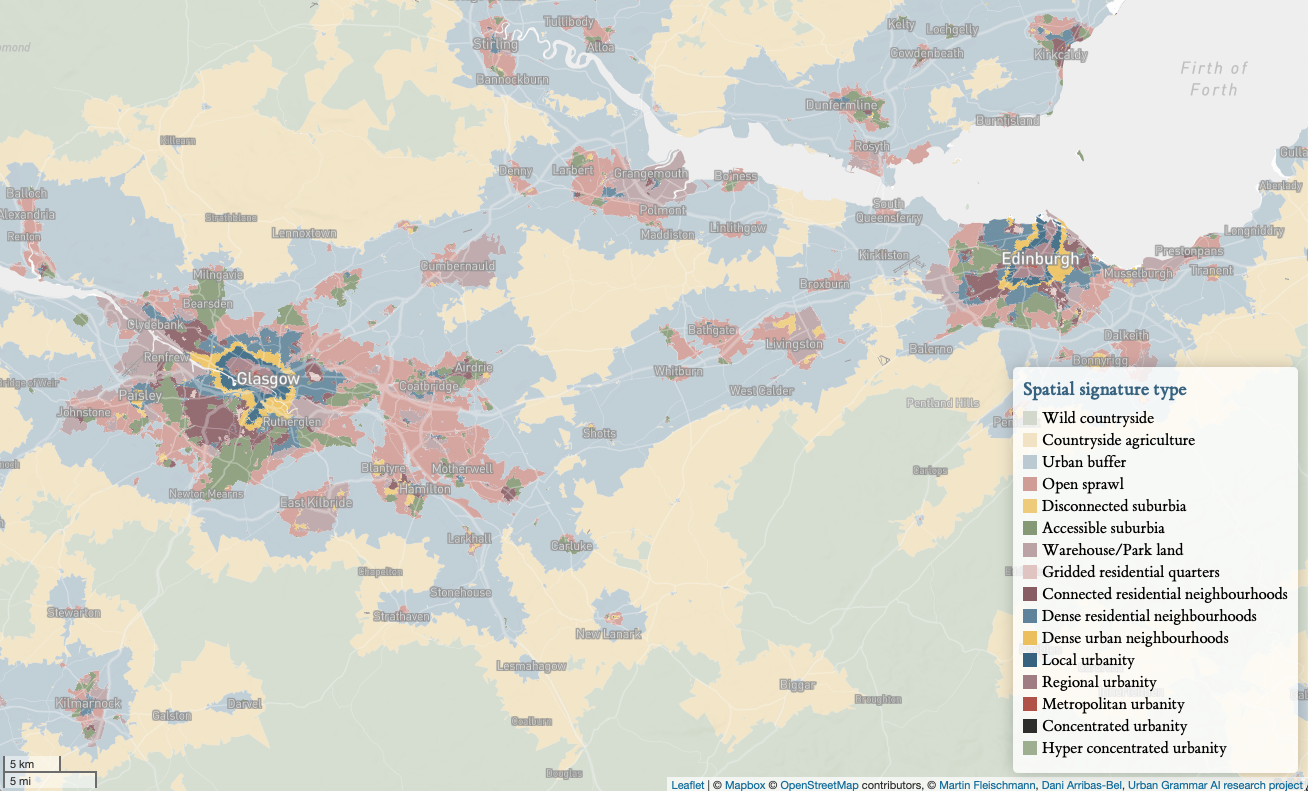
\includegraphics[width=\linewidth]{signatures_scotland.png}
    \caption{Spatial signatures in the area of the Scottish Central Belt stretching from Glasgow to Edinburgh.}
    \label{fig:signatures}
\end{sidewaysfigure}



\subsubsection{Sentinel 2 imagery}

% 250 words

The second data input used in this research is satellite imagery provided by the
Sentinel 2 mission. Specifically, we use the pre-processed cloud-free mosaic of Sentinel
2 released by \cite{CORBANE2020105737}.
The mosaic provides pixel-level composite based on imagery for the period January 2017-
December 2018 at an original resolution of 10 meters per pixel. While Sentinel 2
captures many spectral bands beyond traditional visible red, green and blue (RGB), this
research uses only RGB bands due to its employment of pre-trained neural networks
stemming from non-satellite imagery that is composed only of RGB. The exclusion of other
bands may be seen as a limiting factor of the work, but we believe that, as with other
aspects that will be discussed later, it efficiently illustrates the \textit{lower
bound} of the performance of the presented method and can be only improved with the addition of
other spectral bands or other data (e.g. synthetic-aperture radar imagery).

Another notable aspect of the Sentinel 2 imagery is the resolution. Ten meters per pixel
may be enough to distinguish LULC classes, as shown by the research project discussed
above. However, there is the question of whether it is enough to segment urban
environments. Individual buildings often do not stretch beyond the spatial extent of two
pixels, which is severely limiting what we can \textit{see} on the image, as illustrated
in Figure \ref{fig:signatures}. While other data sources may provide better
resolution\footnote{For example, commercial imagery by Maxar reaches a resolution of
30cm per pixel and imagery by Planet of 50cm per pixel}, potentially improving model
performance, this research is bound within the limits of \textit{open data}, where
Sentinel 2 is the best offering to date.


\subsection{Methods}

% 250 to explain the overarching experiments

We define our challenge as an image classification task and use competing alternatives
to explore which one performs best. Each of them implies geographically relevant
trade-offs. First, we build and train a model composed of a convolutional neural network
and probability modelling able to predict the 12 classes derived from the spatial
signatures. Second, we use methods designed to unveil which of the inherently
geographical decisions being tested has a significant effect on the resulting
performance and should therefore be considered when applying CNN to spatial
problems.

Overall, our exercise is structured as a comparison of models that attempt to
predict the 12 spatial signatures entirely from Sentinel 2 imagery. Each model takes
a set of chips as input runs the class prediction using the convolutional neural
network (CNN) and builds a (spatial) model on top of the resulting probabilities. The
differences between the models are capturing the geographical options being tested - an
extent of the area sampled from the satellite imagery into a single \textit{chip},
presence of spatial augmentation, class exclusivity within each chip, and an
architecture of probability modelling on top of a prediction coming from the CNN.

Finally, the performance of each model is assessed using both traditional non-spatial
techniques used in deep learning and bespoke spatial metrics. Given a large number of
resulting values, a regression approach is used to determine the effect of the tested
options.

Each of the steps is further discussed in detail in the subsequent sections.

\subsubsection{Chip size}

% 500 words

The first question that needs to be answered when trying to apply a classification
algorithm on satellite imagery that spans a large amount of continuous land is how
to sample such data into individual patches (or, hereafter, chips)
that can be assigned to classes. Pre-trained CNNs usually expect a square image of
a certain size, but that does not mean that the same size (in terms of pixels) needs to
be directly sampled from the image, thanks to possible resampling. What should be
retained, though, is the ratio. Therefore, we need to sample square chips of a
custom size. Within an image classification framework, we assume that
each chip contains data of a single class only. Therefore, such a chip should be entirely
within the boundary of a single signature type. That poses some restrictions as spatial
signatures, especially in the urban context, tend to be relatively granular, and large chips
would not fit inside the boundaries, reducing the number of
valid chips for training. Therefore, the goal is to find a balance
between the number of chips sampled from the data and the amount of
information each chip can hold. Given the relatively coarse resolution of Sentinel 2, a
chip of 100x100 meters consists of only 10x10 pixels, which may not be enough to capture
the nature of a signature type and distinguish it from other types. On the other hand, a
chip of 1000x1000 meters, which is likely large enough to capture the difference, will
not fit in most of the signature boundaries and we would end with only a few chips per
urban class.

The literature rarely discusses this decision-making process when defining the chip
size. In some cases, the size is predetermined due to the requirement of either a
pre-trained model or an existing set of labelled data \citep{taubenbock2020}. In
other ones, the size that has
been used in previous studies is applied again without discussing the implications
of such a decision \citep{wang2018mapping}. From a spatial analysis
perspective, this approach is surprising as deciding the chip size is a prime example of the
modifiable areal unit problem (also known as MAUP,
\citealp{openshaw1981modifiable}), especially the aspect about scale, which states that
a change of the scale may affect the outcome of an experiment. Hence such an effect
should be at least considered in an interpretation if not intentionally minimized.

In this work, we try to understand the effect of a chip size by testing all the models
based on four different chip sizes - 80, 160, 320 and 640 meters representing chips of
8x8, 16x16, 32x32 and 64x64 pixels, respectively, illustrated on a Figure \ref{fig:signatures}.


\begin{figure}
    \centering
    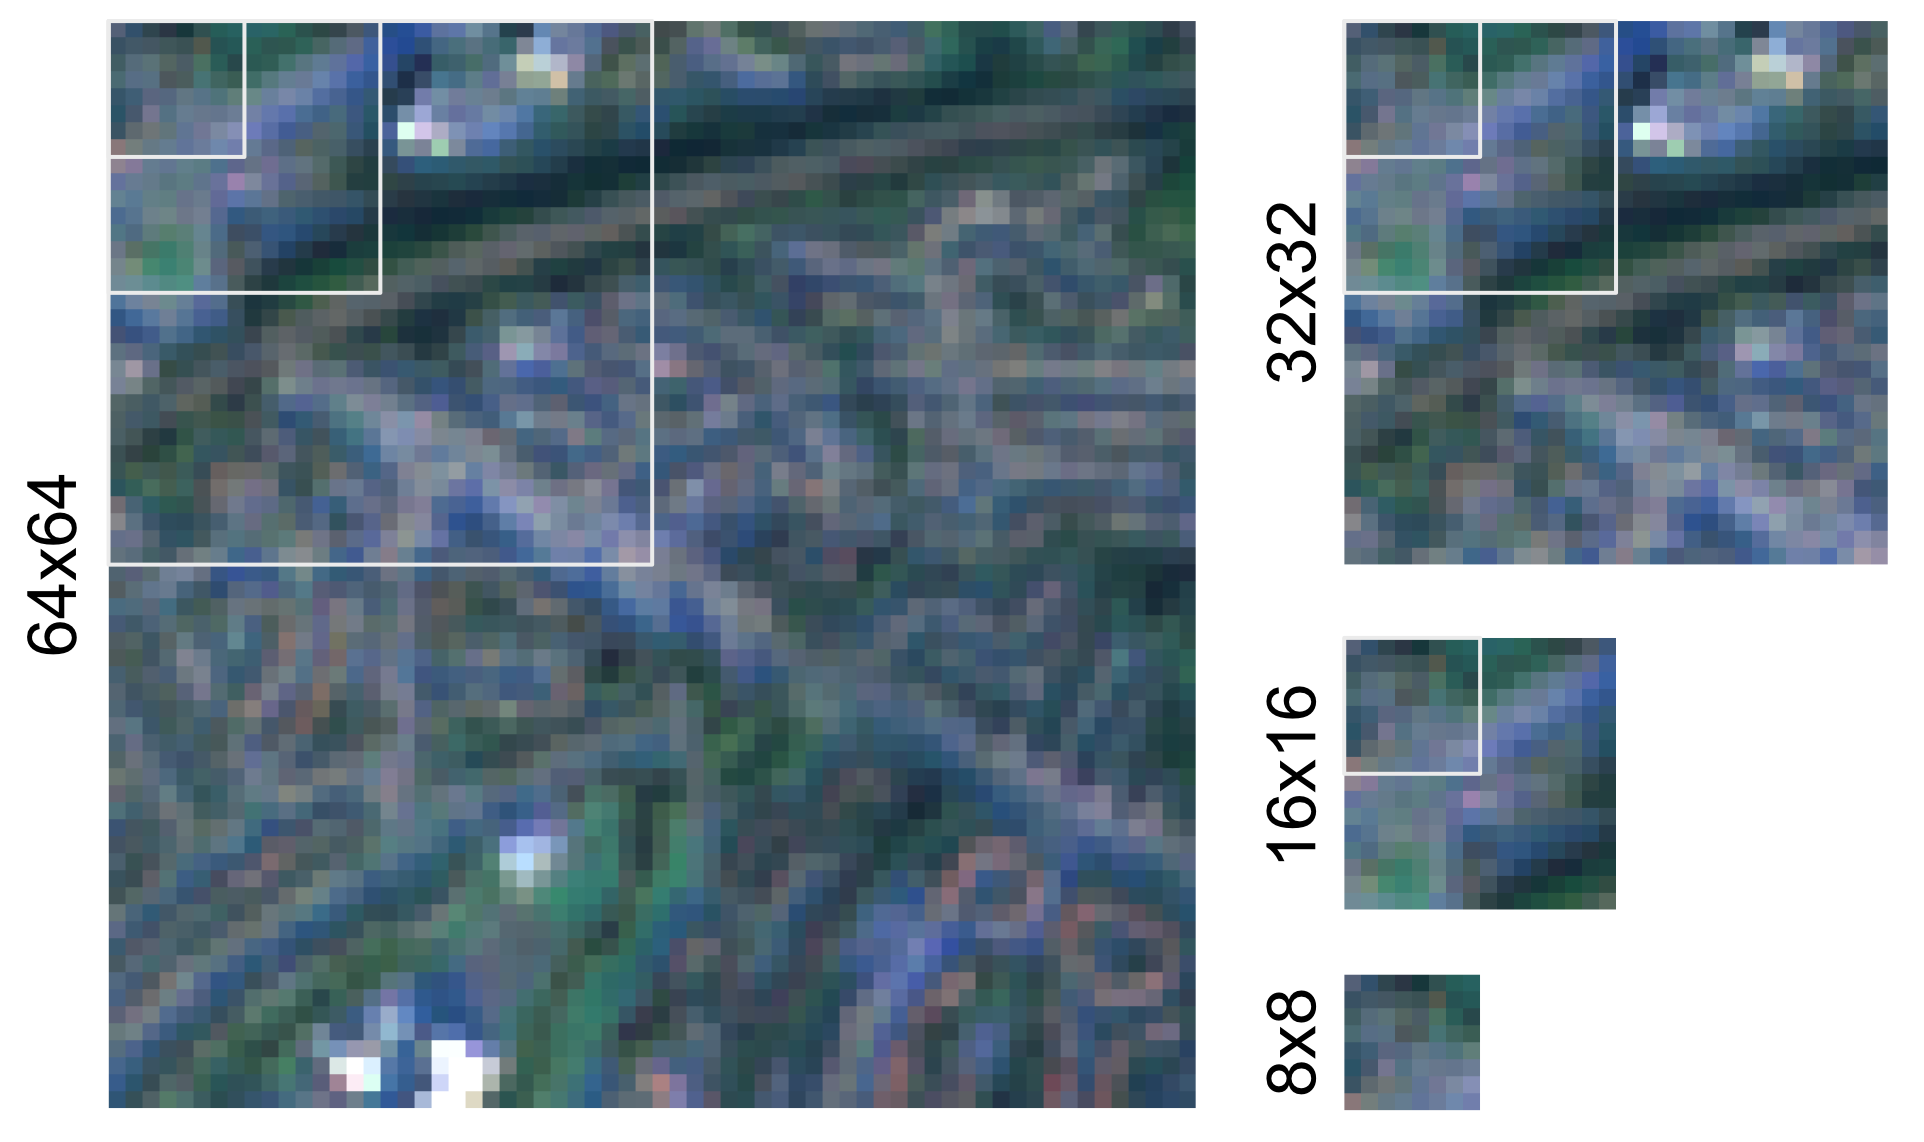
\includegraphics[width=.8\linewidth]{chips.png}
    \caption{Illustration of the selected chip sizes using the Sentinel 2 cloud-free mosaic. Each of the chips also shows the sizes of the smaller options as a white outline.}
    \label{fig:chips}
\end{figure}



\subsubsection{(Spatial) data augmentation - \textit{Sliding}}

% Sliding

% 250 words

As mentioned above, in combination with the signature
geometry and the
the requirement to keep them exclusively within a single class, specific chip sizes may result in
insufficient training data for some signature types. Under-sampling like this
one can be a serious problem that is not unique to spatial modelling. However,
traditional augmentation methods are not directly applicable here. For example, in an
image classification problem trying to determine if there is a cat or a dog on an image,
we can flip the picture along the y-axis, add some rotation or zoom to get more versions of
the same image and expand the set of training data. Neither of these methods is
applicable to spatial problems. Flipping or rotating the image would break
natural light conditions, while zooming in would change the scale of the urban environment
we attempt to capture.

At the same time, the geographical and continuous nature of the data at hand
allows us to use explicitly spatial augmentation techniques such as the one we
call \textit{sliding}.
Sliding can be seen as overlapping sampling. Instead of overlaying a grid of chips over
target geometry and using each pixel only once, we take the initial grid and slide it a
few pixels horizontally and vertically, as illustrated in Figure \ref{fig:sliding}. If
the boundary of a slid chip is fully within a signature geometry, it is added to the
pool of chips to be used. This process is done repeatedly to ensure that each class has
a reasonable amount of chips to work with.

It is to be noted that sliding can cause a data leakage (sequences of pixels being
present in both training and validation) if done before splitting the data into
training and validation subsets. Therefore, we first create the initial grid, subdivide
it spatially into four parts (40\% for CNN training, 10\% for CNN validation, 40\% for
probability modelling training, 10\% for probability modelling validation) and apply
sliding within each part to avoid any pixels being shared among chips from different
sets. Subdivision into the four parts is done within each signature geometry to avoid
potential geographical bias.

\begin{figure}
    \centering
    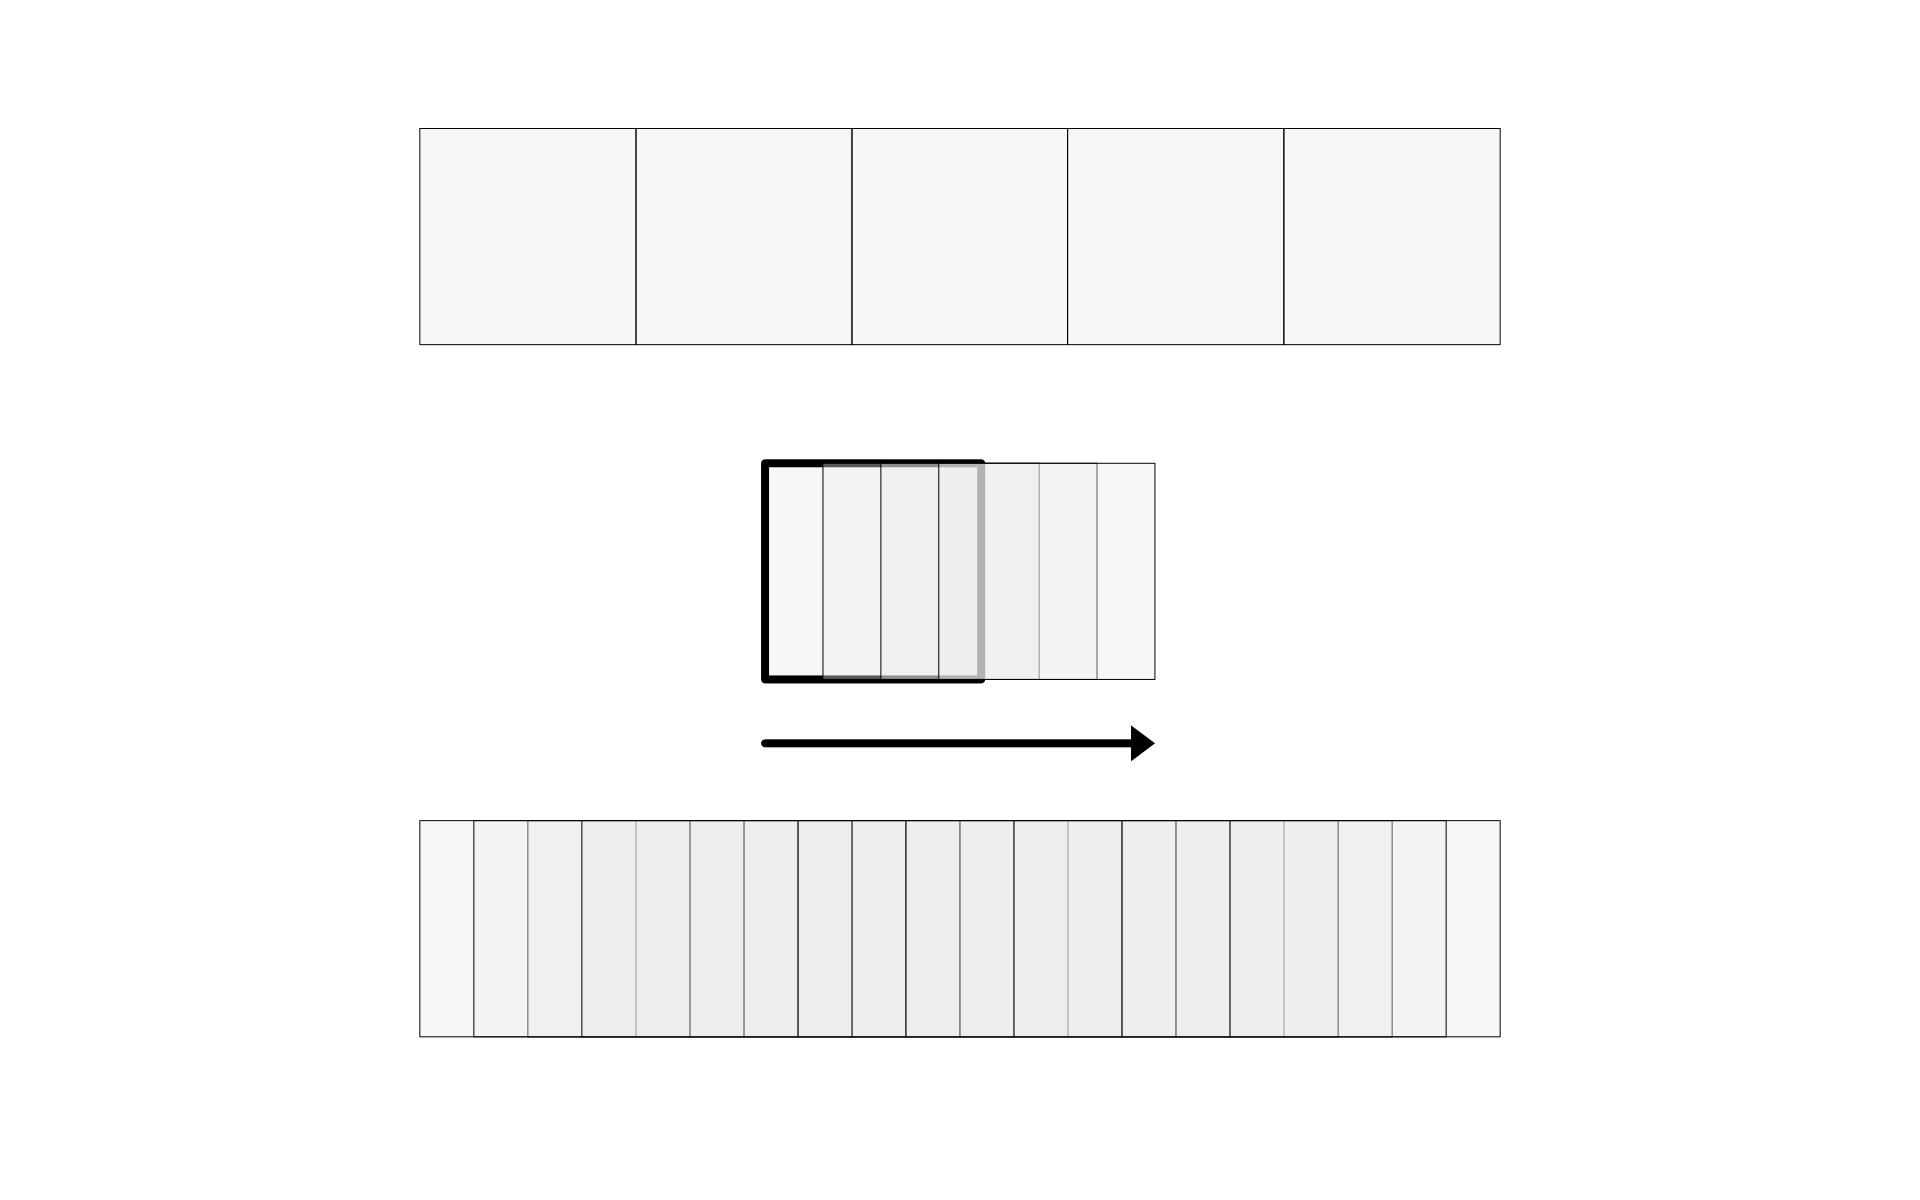
\includegraphics[width=.8\linewidth]{sliding.png}
    \caption{Diagram illustrating the sliding mechanism in one direction. The first row shows the initial non-overlapping grid, the last one final overlapping set of chips. The same approach is then also applied vertically.}
    \label{fig:sliding}
\end{figure}


\subsubsection{Model architecture}

% 500 words

% Overall content of the section

Model architecture refers to the analytical pipeline that transforms chips
into a prediction for a single signature type. Our competing architectures
contain two main parts. First is a CNN that transforms a single chip into a
set of 12 probabilities, one for each signature type.
Second is a mathematical function that converts such probabilities (
considering only those for the chip of interest or in conjunction with
those of neighbouring chips) into a
prediction for a single signature type. This section describes each of these in detail.
We would like to highlight that, contrary to the majority of deep
learning-focused research, our focus is not on the architecture of the CNN
itself. We assume the effect of geographic choices will largely show similar
behaviour irrespective of the network architecture. For that reason, throughout
our experiments we use \texttt{EfficientNetB4} \citep{https://doi.org/10.48550/arxiv.1905.11946}, pre-trained
on the popular ImageNet dataset \citep{deng2009imagenet}. Appendix \ref{sec:appendixA} shows a brief comparison of
several standard neural network architectures and their performance on a subset of data
to motivate our decision. We then apply transfer learning by re-training the
top layer of the pre-trained model and replacing it by a
custom sequence of dense layers described below.

% Standard image classification
We consider three variants of the CNN.
The default approach (which we will refer to \texttt{bic}, for ``baseline
image classification'') is a standard image classification problem, using the sets of chips
that are fully within a single signature type. The custom top layer of the pre-trained CNN then contains a Global Average
Pooling (2D) layer, a dense layer with ReLu activation and 256 neurons, and a dense
layer with the softmax activation and a number of neurons equal to a number of classes
(12). A result for a single chip is a collection of 12 probabilities
of a chip belonging to each signature type. The sum of all probabilities is
one.
An extension of this approach (\texttt{sic}, for ``sliding image
classification'') applies this technique to the data being spatially augmented
with the sliding technique described above.

% Multi-output regression
Our third approach recasts the image classification task as a multiclass
prediction. If we relax the requirement that every chip is fully within
the boundaries of a single signature type, we end up with many more available
chips, but now some of them include more than a single label within their
extent. Instead of a single label per chip, we now deal with a 1-D array of them.
This can be beneficial from the geographical perspective as such chips now inherently
encode the co-location of individual signature types and a model could use this information
during the prediction. As signature types usually tend to neighbour only a subset of
other classes (e.g., Urbanity never neighbours Wild Countryside), we can assume that
information on co-location can positively impact predictive performance. We
then include a set of chips sampled from a grid crossing the boundaries of
signature types (using the same chip sizes as before) and adapt the CNN to
perform multi-output regression (\texttt{mor}) instead of image classification. This change
implies the top layer is now composed of a Global Average Pooling (2D) layer, a
dense layer with ReLu
activation and 256 neurons, and a dense layer with the sigmoid activation and a number of
neurons equal to a number of classes (i.e., 12). The result for a single chip is a similar
collection of probabilities, but these are now predicted proportions. As such,
the sum of all of them ranges between 0 and 12 rather than between 0 and 1.

% Spatial modelling of probabilities TODO: Dani, from this section below are your bits.
The second step in the pipeline takes chip probabilities and turns them into
predictions of a signature type. To do this, we compare five approaches of
differing complexity and sophistication. These five variants stem from the
combination of two components: the set of inputs used to make the prediction and
the function transforming them into a single signature type. For a given chip
$i$, we can express this step of the pipeline mathematically as follows:

\begin{equation}
\begin{split}
        S_i & = f(P) \\
        P & = \underbrace{
                \sum_{k} P_{k-i}
        }_\text{baseline}\;
        \underbrace{
        \left[+ \sum_{k} \sum_j w_{ij} P_{k-j}\right]
}_\text{wx}
        \label{eq:sp_model}
\end{split}
\end{equation}

where $S_i$ is the prediction for the signature type of chip $i$ (one of the $k$ available, where
$k=12$ in our case) and $f(\cdot)$ is a function that
transforms the inputs $P$ into $S_i$. The five
approaches we compare derive from the different implementations of $f(\cdot)$
and $P$. On the latter, we compare models that only use the probabilities
$P_{k-i}$ generated by the CNN for chip $i$ (\texttt{baseline}) with alternatives
(signalled with the \texttt{wx} term) that, in addition,
also include an average of $P_{k-j}$ probabilities, which are the
probabilities generated by the CNN for each neighbour $j$ of chip $i$. This is
akin to what in spatial analysis is called the \textit{spatial lag} of each
probability, and is calculated using a spatial weights matrix $W$ that records
the spatial relationship between every chip in the set. In our $W$, two
neighboring locations $i$ and $j$ will receive a weight $w_{ij}=1$,
if they are in the same of the four split sets as defined above, and if they
either are geographically contiguous or are nearest neighbours; while otherwise
they will be considered non-neighbours and receive a weight $w_{ij}=0$. To obtain
an average of the neighbors, we row-standardise $W$ so that $\sum_j w_{ij} =
1$. The second dimension other than $P$ we vary is the function $f(\cdot)$ that converts
it to the prediction $S_i$. We take three distinct approaches here: simply
picking the maximum probability (\texttt{maxprob}), which we only use without the spatial lag of
probabilities; an ensemble of binary logit models to predict each class
(\texttt{logite}), then selecting the class with top probability, which we
also use with the \texttt{wx} variant; and a histogram-based gradient boosted
classifiers inspired by LightGMB \citep{ke2017lightgbm} and implemented in
\texttt{scikit-learn} \citep{pedregosa2011scikit}. This yields our five
competing models:
\texttt{maxprob}, \texttt{logite\_baseline}, \texttt{logite\_baseline-wx},
\texttt{HGBC\_baseline}, and \texttt{HGBC\_baseline-wx}.

\subsubsection{Performance metrics}

% 500 words
The goal of our experiments is to compare different models under varying
geographical conditions to learn both which performs best, but also how
different choices of geographical nature influence the overall performance
when predicting form and function from satellite imagery.
To provide a workbench that systematically compares each model and setup, we
use a set of performance scores that operate either at the global or class level,
and that measure performance in the traditional machine learning sense, as
well as in the spatial sense.

% Traditional non-spatial
We use four standard performance scores. \textit{Cohen's kappa} score ($\kappa$,
\citealp{cohen1960coefficient}) is a measure of agreement between two sets of
categorical labels that ranges from -1 to 1. Intuitively, it measures the
extent to which the two sets agree with each other (i.e., same label for the
same observation) beyond what would be expected from pure chance
($\kappa=0$). Cases where there is more disagreement than expected from chance
receive a negative score. \textit{Global (within-class) accuracy} captures the
proportion of observations correctly predicted (in a given class). The
\textit{Macro F1} is a score that aggregates class-based F1
scores. The F1 is the harmonic mean between precision (proportion of
chips predicted in one class actually belonging to that class) and recall
(proportion of chips belonging to a given class being predicted as such).
We use both the \textit{weighted Macro F1} as well as the \textit{averaged
Macro F1}. The latter takes the standard mean of the F1 scores for each class,
while the former weights each F1 by the proportion of chips in each class.

% Explicitly spatial metrics % Why % Which ones % Why those? (ideally link to Miguel's
%paper suggestions)
In addition to traditional performance scores, we also evaluate how similar
the spatial pattern of predictions is to that of the original labels.
The measures described above are all ``spatially unaware'' in the sense that
they quantify different aspects of the correctness of a model's
predictions but ignore their spatial patterning. Two
sets of results may have the same amount of correct predictions, but in one,
the spatial layout of such predictions may be close to
that of the observed labels, while the other one spatially allocates mispredictions in
a way that differs more from what is observed empirically. Given the nature of
our classification challenge --identify form and
function over space from satellite imagery-- the spatial dimension of model
performance is of great importance. Since the spatial signatures represent a
set of (12) distinct categories, we rely on the \textit{join counts} statistic
(JC, \citealp{cliff1981spatial}). The JC measures the degree of spatial
concentration in a binary categorical variable; hence, we use it at the class
level. For each class in each model, we retain the proportion of pairs of
chips in the same class that are spatial neighbours (``joins'') over the total number of
pairs that are spatial neighbours.
Our neighbourhood definition relies on two alternative spatial weights matrices:
one based on a distance threshold of $1Km$ ($W_{thr}$), and one that combines
the nearest neighbour with those defined by contiguity ($W_{union}$).
Our metric of interest is then the error (i.e., absolute
value of the difference) between this proportion for the model of interest and
that of the observed labels.

\subsubsection{Summarizing experiments}

% 250 words

The setup described above generates over 60 different
models to be trained to predict 12 signature types and six performance measures
to evaluate them. Making sense of their results requires a
systematic approach that summarises them and provides explicit tests for the
questions we are trying to answer. We achieve this goal by fitting linear
regressions that explain performance scores for each model as a function
of the characteristics of the setup evaluated. Specifically, we estimate the
following two equations. First, for global scores, we run:

\begin{equation}
        Perf_i = \alpha +
        \sum_m \delta_m M_i +
        \sum_a \gamma_a A_i +
        \beta_1 Chip \; Size_i +
        \beta_2 W_i +
        \epsilon_i
        \label{eq:reg_global}
\end{equation}


where $Perf_i$ is each of our four global performance scores measured for trained
model in setup $i$; $\alpha$ is an intercept; $M_i$ are indicator variables for the
type of model we estimate (i.e., \texttt{maxprob}, \texttt{logite},
\texttt{HGBC});\footnote{We remove \texttt{HGBC} to avoid perfect
collinearity and hence treat it as the reference model.} $A_i$ are,
similarly, indicator variables for the architecture used (i.e.,
\texttt{bic}, \texttt{sic}, \texttt{mor});\footnote{We remove \texttt{BIC} to avoid perfect
collinearity and hence treat it as the reference model.} $Chip \; Size_i$
captures the number of pixels the chips in the setup contain; $W_s$ is another
indicator variable that takes the value of one if the model includes the
spatial lag of signature type probabilities and zero otherwise;
and $\epsilon_i \sim \mathcal{N}(0, \sigma)$ is an i.i.d. error term.

Second, for class-based scores, we fit:

\begin{equation}
        Perf_{i-s} = \alpha +
        \sum_m \delta_m M_i +
        \sum_a \gamma_a A_i +
        \beta_1 Chip \; Size_i +
        \beta_2 W_i +
        \beta_3 \left[\%\right]Obs_{i-s} +
        \sum_s \zeta_s S_{i-s} +
        \epsilon_{i-s}
        \label{eq:reg_class}
\end{equation}

where $\left[\%\right]Obs$ represents either the number of chips in
signature $s$ in setup $i$ or as a proportion of the total; and $S_{i-s}$ an
indicator variable for the signature type $s$;\footnote{We remove
\texttt{Accessible suburbia} to avoid perfect collinearity and hence treat it
as the reference model.} and the rest is as in Equation \ref{eq:reg_global}.
%
Importantly for both equations,
$\delta_m/\gamma_a/\beta_1/\beta_2/\beta_3/\zeta_s$, parameters to be
estimated by the regression model, provide a direct and formal test to the key
questions we set out to answer with our experiments.

\section{Results} % 500 words in total
\label{sec:results}

% Overview of numbers


% figure 1 - within class accuracy per model
Within-class accuracy by the model can be seen in Figure \ref{fig:wc_accuracy_x_model} (a
sister figure where scores are grouped by signature rather than by model can be found in
Appendix \ref{sec:appendixB}). We can notice some consistent patterns already. The
baseline image classification (\texttt{bic}) tends to underperform other architectures,
especially on more urban signature types. On the other hand, multi-output regression (\texttt{mor}),
using the larger chip size (32 or 64), tends to show the highest values across signature
types and models. If we look at accuracy for individual signature types, both extremes
(urbanity on one side and both countryside classes on the other)
tend to be the easiest to predict. Regarding the models, there is no immediate conclusion to be
made apart from a clear indication that the maximum probability (\texttt{maxprob}) approach is generally
worse than any of the modelling, suggesting that there is a value in the modelling step.
The within-class accuracy can be further explored using confusion matrices available as an
Appendix \ref{sec:appendixC}.


\begin{sidewaysfigure}
    \centering
    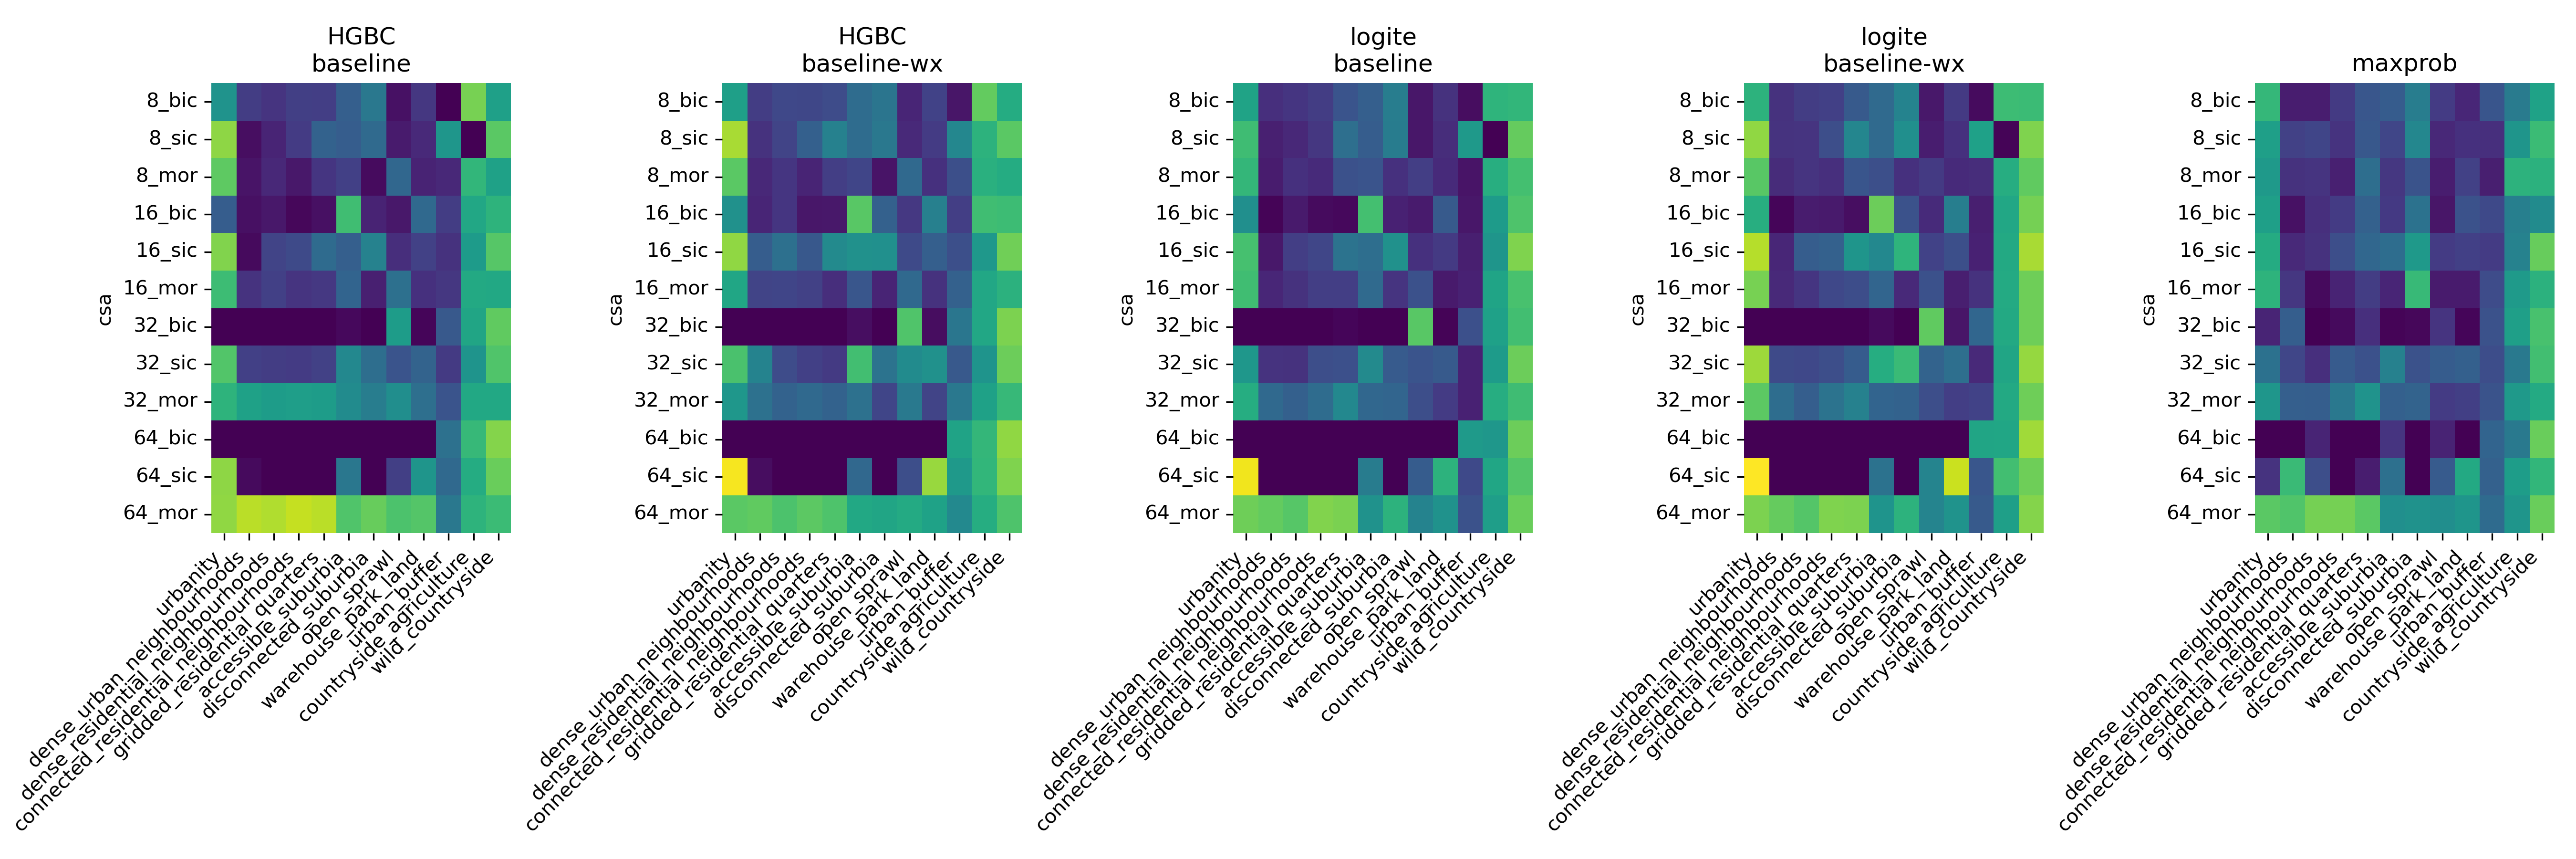
\includegraphics[width=1.0\linewidth]{wc_accuracy_x_model.png}
    \caption{Within-class accuracy scores grouped by model. Each panel
    represents results from one of the five models compared, namely:
    histogram-based boosted classifier (\texttt{HGBC}) with features
    pertaining only to a given chip (\texttt{baseline}) or including also features
    from neighbouring ones (\texttt{baseline-wx}); Logit ensemble
    (\texttt{logite}) with the same two variations; and a simpler maximum
    probability approach (\texttt{maxprob}). Each row in the heatmap
    corresponds to a pair of chipsize (8, 16, 32, and 64 pixels)
    and architechture (baseline image classification, or \texttt{bic}; sliding
            image classification, or \texttt{sic}; and multi-output
    regression, or \texttt{mor}) used in the neural network stage of the
    pipeline. Colouring is standardised across panels and values range from
    0 (dark purple) to 1 (bright yellow).}
    \label{fig:wc_accuracy_x_model}
\end{sidewaysfigure}

Whilst plotting the accuracy is a way to build an intuition about the performance of
individual options, it does not quantify their effects. The linear regressions shown in
tables \ref{tab:non_sp_reg} and \ref{tab:non_sp_reg_wc} provide a better insight. The
first regression explains global performance scores (Cohen's kappa, Global Accuracy, Marco F1
weighted and Macro F1 average). We can draw a few conclusions from this. First, the chip size
seems to have a positive effect on the results, as it is consistently
significant across all metrics. Except for the average macro F1 score, there is a
positive effect of the inclusion of spatial lag in the modelling step (W). Regarding the
CNN step, we do not see a lot of significance but there are indications that sliding
image classification and multi-output regression approaches outperform baseline image
classification. Comparing the probability modelling step, we see an indication that the
maximum probability is the least performant of the options, again suggesting the value
of the modelling.


% table 1 non spatial, one col for regression
\begin{table}
        \centering
\begin{tabular}{lcccc}
\toprule
{} &    $\kappa$ & Global Accuracy & Macro F1 w. & Macro F1 avg. \\
\midrule
Intercept                                         &  0.2185*** &        0.3236*** &    0.2790*** &      0.1798*** \\
                                                  &   (0.0209) &         (0.0175) &     (0.0174) &       (0.0375) \\
(M) Logit E.                                       &    -0.0245 &         -0.0256* &    -0.0324** &        -0.0325 \\
                                                  &   (0.0168) &         (0.0141) &     (0.0141) &       (0.0302) \\
(M) Max. Prob.                                     &  -0.0559** &       -0.0606*** &    -0.0421** &        -0.0296 \\
                                                  &   (0.0222) &         (0.0187) &     (0.0186) &       (0.0399) \\
(A) M.O.R.                                         &     0.0227 &        -0.0357** &     -0.0278* &      0.1787*** \\
                                                  &   (0.0184) &         (0.0155) &     (0.0154) &       (0.0331) \\
(A) S.I.C.                                         &     0.0232 &          -0.0247 &      -0.0171 &      0.1101*** \\
                                                  &   (0.0184) &         (0.0155) &     (0.0154) &       (0.0331) \\
Chip Size                                         &  0.0036*** &        0.0043*** &    0.0048*** &       0.0014** \\
                                                  &   (0.0004) &         (0.0003) &     (0.0003) &       (0.0006) \\
W                                                 &  0.0572*** &        0.0468*** &    0.0531*** &         0.0392 \\
                                                  &   (0.0168) &         (0.0141) &     (0.0141) &       (0.0302) \\
\midrule
$R^2$                                             &     0.7214 &           0.8281 &       0.8514 &         0.4191 \\
$R^2$ Adj.                                        &     0.6899 &           0.8086 &       0.8346 &         0.3533 \\
N.                                                &     60     &           60     &       60     &         60     \\
\bottomrule
\end{tabular}
    \caption{\label{tab:non_sp_reg}Regression outputs explaining
            global non-spatial
    performance scores. Explanatory variables with a preceding (M) and (A)
    correspond to binary variables for the type of model (with histogram-based
            boosted classifier, or \texttt{HGBC}, as the
    baseline) and architecture (with baseline image classification, or
    \texttt{BIC}, as the baseline),
    respectively. Standard errors in parenthesis. Coefficients significant at
    the 1\%, 5\%, 10\% level are noted with ***, **, and *, respectively.}
\end{table}

The table \ref{tab:non_sp_reg_wc} then looks again at the within-class accuracy explaining
what we have seen in figure \ref{fig:wc_accuracy_x_model}. The
multi-output regression consistently outperforms both baseline image classification and
sliding image classification (which shows inconsistent results itself). Chip size has,
again, a positive effect on the performance, while the inclusion of spatial
lag in the modelling also consistently shows a positive impact. As assumed above, the
prediction of signature types on both extremes of the urban-wild range tends to be
easier than classes in between.

\begin{table}
\begin{tabular}{lccc}
\toprule
{}  &       \multicolumn{3}{c}{Within-Class Accuracy} \\
\midrule
Intercept                                         &   0.1866*** &     -0.0237 &    0.0595** \\
                                                  &    (0.0308) &    (0.0311) &    (0.0303) \\
(M) Logit E.                                      &     -0.0125 &     -0.0125 &     -0.0125 \\
                                                  &    (0.0159) &    (0.0141) &    (0.0146) \\
(M) Max. Prob.                                    &     -0.0188 &     -0.0188 &     -0.0188 \\
                                                  &    (0.0211) &    (0.0186) &    (0.0193) \\
(A) M.O.R.                                        &   0.1753*** &   0.2512*** &   0.1753*** \\
                                                  &    (0.0175) &    (0.0163) &    (0.0160) \\
(A) S.I.C.                                        &   0.1202*** &  -0.0783*** &   0.1202*** \\
                                                  &    (0.0175) &    (0.0209) &    (0.0160) \\
Chip Size                                         &   0.0014*** &   0.0041*** &   0.0014*** \\
                                                  &    (0.0003) &    (0.0003) &    (0.0003) \\
1k Obs.                                           &             &   0.0514*** &             \\
                                                  &             &    (0.0036) &             \\
\% Obs.                                           &             &             &   0.0156*** \\
                                                  &             &             &    (0.0013) \\
W                                                 &    0.0365** &   0.0365*** &    0.0365** \\
                                                  &    (0.0159) &    (0.0141) &    (0.0146) \\
(S)Urbanity                                       &   0.2358*** &   0.2022*** &   0.2574*** \\
                                                  &    (0.0349) &    (0.0309) &    (0.0320) \\
(S)Dense urban neighbourhoods                     &  -0.1420*** &  -0.1075*** &  -0.0998*** \\
                                                  &    (0.0349) &    (0.0309) &    (0.0322) \\
(S)Dense residential neighbourhoods               &  -0.1414*** &  -0.0836*** &  -0.0983*** \\
                                                  &    (0.0349) &    (0.0311) &    (0.0322) \\
(S)Connected residential neighbourhoods           &  -0.1306*** &   -0.0726** &   -0.0754** \\
                                                  &    (0.0349) &    (0.0311) &    (0.0323) \\
(S)Gridded residential quarters                   &   -0.0785** &     -0.0127 &     -0.0049 \\
                                                  &    (0.0349) &    (0.0312) &    (0.0326) \\
(S)Disconnected suburbia                          &    -0.0601* &     -0.0103 &     -0.0019 \\
                                                  &    (0.0349) &    (0.0311) &    (0.0324) \\
(S)Open sprawl                                    &   -0.0845** &  -0.0995*** &  -0.1143*** \\
                                                  &    (0.0349) &    (0.0309) &    (0.0321) \\
(S)Warehouse park land                            &   -0.0857** &   -0.0788** &   -0.0817** \\
                                                  &    (0.0349) &    (0.0309) &    (0.0320) \\
(S)Urban buffer                                   &   -0.0828** &  -0.1382*** &  -0.1753*** \\
                                                  &    (0.0349) &    (0.0311) &    (0.0330) \\
(S)Countryside agriculture                        &   0.2236*** &   0.1593*** &   0.1118*** \\
                                                  &    (0.0349) &    (0.0312) &    (0.0334) \\
(S)Wild countryside                               &   0.3876*** &   0.3283*** &   0.2925*** \\
                                                  &    (0.0349) &    (0.0311) &    (0.0330) \\
\midrule
$R^2$                                             &      0.4979 &      0.6087 &      0.5794 \\
$R^2$ Adj.                                        &      0.4857 &      0.5987 &      0.5686 \\
N.                                                &      720    &      720    &      720    \\
\bottomrule
\end{tabular}
    \caption{\label{tab:non_sp_reg_wc}Regression outputs explaining
            within-class accuracy. Explanatory variables with a preceding (M),
            (A) and (S)
    correspond to binary variables for the type of model (with histogram-based
            boosted classifier, or \texttt{HGBC}, as the
    baseline), architecture (with baseline image classification, or
    \texttt{BIC}, as the baseline) and spatial signature (with Accessible
    suburbia as the baseline),
    respectively. Standard errors in parenthesis. Coefficients significant at
    the 1\%, 5\%, 10\% level are noted with ***, **, and *, respectively.}
\end{table}

% figure 2 - map for a single class target/prediction/

%       \begin{figure}
%           \centering
%           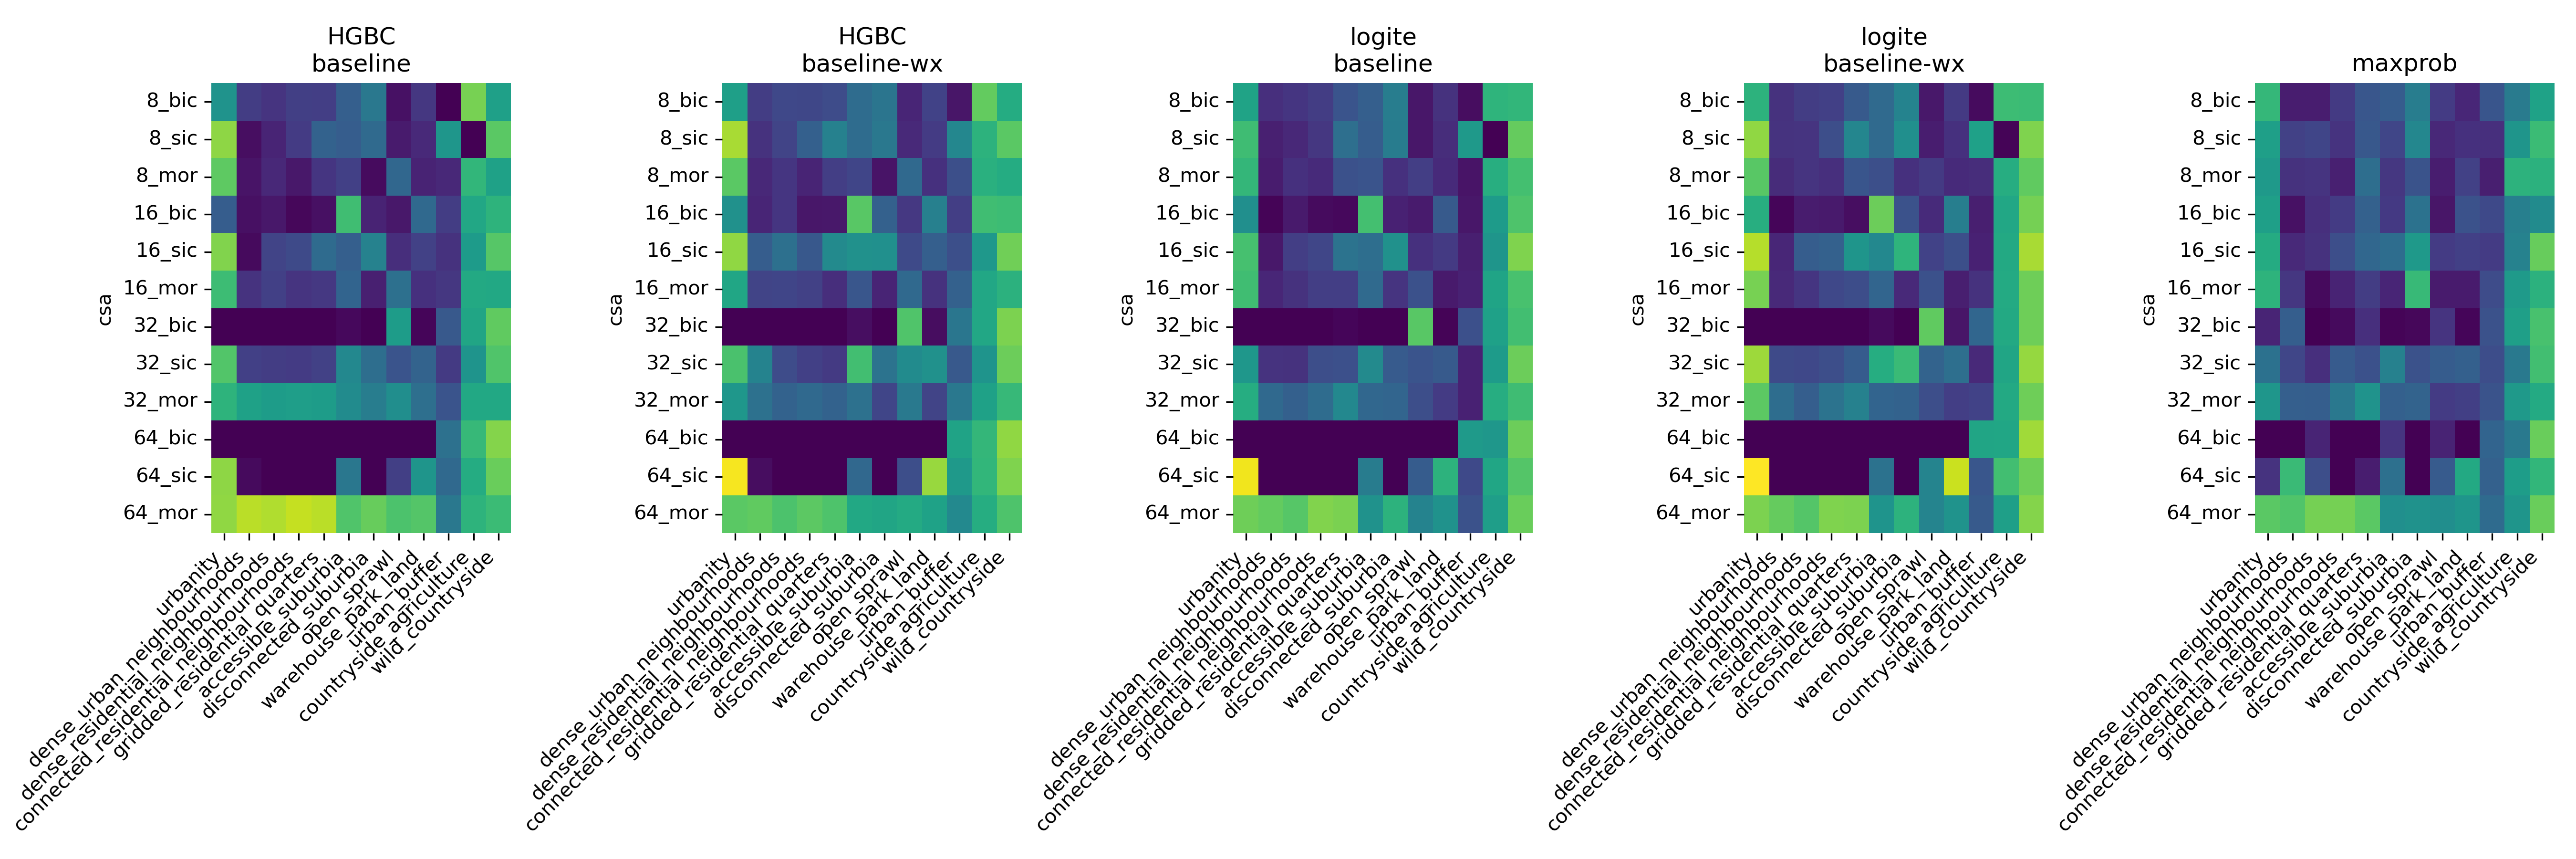
\includegraphics[width=1.0\linewidth]{wc_accuracy_x_model.png}
%           \caption{TBC}
%           \label{fig:prediction_comparison_maps}
%       \end{figure}
% DAB: for space constraints, we have decided to drop it for now

The regression outputs explaining differences in the spatial pattern between observed
and predicted values measured by the Join Counts statistic offer another - spatially
explicit - perspective on the performance of tested model configurations. As such, it
also indicates slightly different results as presented in the table \ref{tab:sp_reg_wc}.
Neither option of the probability modelling steps seem to have a significant effect on
the Join Counts results, unlike in previous performance metrics. However, the
architecture of the neural network step shows a significant effect as multi-output
regression, and in two out of four cases also sliding image classification, outperform the
baseline image classification. While the effect of the chip size is inconsistent across the
options, the inclusion of the spatial lag in the modelling step has a significant effect (at
either 10\%, 5\% or 1\% significance level). The effect of a signature type depends on
its nature. More compact urban types like \textit{Urbanity} and \textit{Dense
urban neighbourhoods} show significance when using a distance threshold spatial weights,
while sparser signature types like \textit{Open Sprawl} and \textit{Urban Buffer} show
significance when using a union of weights.


% table 2 spatial,

\begin{table}
        \begin{tabular}{lcccc}
                \toprule
                {} &  $JC$ & $\log(JC)$ & $JC$  & $\log(JC)$  \\
                {} &  $W\_{thr}$ &  $W\_{thr}$ &  $W\_{union}$ &  $W\_{union}$ \\
                \midrule
                Intercept                                         &   4.3454*** &       1.4617*** &    4.7103*** &         1.6311*** \\
                                                                  &    (0.9507) &        (0.1344) &     (0.5763) &          (0.1080) \\
                (M) Logit E.                                      &     -0.1406 &         -0.0431 &       0.1851 &            0.0481 \\
                                                                  &    (0.4951) &        (0.0700) &     (0.2995) &          (0.0561) \\
                (M) Max. Prob.                                    &      0.1128 &         -0.1223 &       0.2819 &            0.0223 \\
                                                                  &    (0.6442) &        (0.0911) &     (0.3887) &          (0.0728) \\
                (A) M.O.R.                                        &  -3.1630*** &      -0.5744*** &   -2.7875*** &        -0.4647*** \\
                                                                  &    (0.5494) &        (0.0777) &     (0.3301) &          (0.0619) \\
                (A) S.I.C.                                        &      0.0119 &      -0.2390*** &    -0.6666** &           -0.0481 \\
                                                                  &    (0.5532) &        (0.0782) &     (0.3329) &          (0.0624) \\
                Chip Size                                         &   0.0297*** &         -0.0005 &      -0.0061 &        -0.0080*** \\
                                                                  &    (0.0108) &        (0.0015) &     (0.0065) &          (0.0012) \\
                W                                                 &    -0.9325* &       -0.1376** &   -0.9556*** &        -0.1785*** \\
                                                                  &    (0.4945) &        (0.0699) &     (0.2991) &          (0.0560) \\
                (S)Urbanity                                       &   4.6650*** &       0.6574*** &       0.1156 &           -0.1258 \\
                                                                  &    (1.0696) &        (0.1512) &     (0.6460) &          (0.1211) \\
                (S)Dense urban neighbourhoods                     &     1.7796* &       0.5094*** &       0.7480 &            0.1609 \\
                                                                  &    (1.0695) &        (0.1512) &     (0.6487) &          (0.1216) \\
                (S)Dense residential neighbourhoods               &     -0.8545 &          0.0672 &      -0.4636 &           -0.0920 \\
                                                                  &    (1.0958) &        (0.1550) &     (0.6647) &          (0.1246) \\
                (S)Connected residential neighbourhoods           &     -0.3656 &          0.1543 &      -0.4388 &           -0.1447 \\
                                                                  &    (1.1018) &        (0.1558) &     (0.6647) &          (0.1246) \\
                (S)Gridded residential quarters                   &     -0.2000 &          0.1009 &      -0.6203 &          -0.2111* \\
                                                                  &    (1.0744) &        (0.1519) &     (0.6517) &          (0.1221) \\
                (S)Disconnected suburbia                          &     -0.9752 &         -0.1719 &      -1.0303 &        -0.3358*** \\
                                                                  &    (1.1213) &        (0.1586) &     (0.6684) &          (0.1252) \\
                (S)Open sprawl                                    &     1.8342* &          0.1734 &    2.1575*** &         0.3576*** \\
                                                                  &    (1.0604) &        (0.1499) &     (0.6432) &          (0.1205) \\
                (S)Warehouse park land                            &      0.5496 &          0.2123 &      1.2245* &          0.3054** \\
                                                                  &    (1.0694) &        (0.1512) &     (0.6487) &          (0.1216) \\
                (S)Urban buffer                                   &     -0.0558 &         -0.0931 &    2.7027*** &         0.5164*** \\
                                                                  &    (1.0521) &        (0.1488) &     (0.6382) &          (0.1196) \\
                (S)Countryside agriculture                        &     -1.3759 &        -0.2511* &       0.6623 &            0.0670 \\
                                                                  &    (1.0521) &        (0.1488) &     (0.6382) &          (0.1196) \\
                (S)Wild countryside                               &    -2.0183* &      -0.5065*** &      -0.5918 &           -0.1635 \\
                                                                  &    (1.0521) &        (0.1488) &     (0.6382) &          (0.1196) \\
\midrule
                $R^2$                                             &      0.1589 &          0.1954 &       0.2118 &            0.2660 \\
                $R^2$ Adj.                                        &      0.1368 &          0.1743 &       0.1913 &            0.2468 \\
                N.                                                &      665    &      665        &   670        &     670           \\
                \bottomrule
                \end{tabular}
    \caption{\label{tab:sp_reg_wc}Regression outputs explaining
            (log of) differences in the spatial pattern between observed and predicted values,
            as measured by the Join Counts statistic. The Join Counts for each signature were computed
            using two types of spatial weights: one based on a distance threshold of 1Km ($W\_{thr}$),
            and another one built as a the union of nearest neighbor and queen contiguity matrices ($W\_{union}$).
            Explanatory variables with a preceding (M), (A) and (S)
    correspond to binary variables for the type of model (with histogram-based
            boosted classifier, or \texttt{HGBC}, as the
    baseline), architecture (with baseline image classification, or
    \texttt{BIC}, as the baseline) and spatial signature (with Accessible
    suburbia as the baseline),
    respectively. Standard errors in parenthesis. Coefficients significant at
    the 1\%, 5\%, 10\% level are noted with ***, **, and *, respectively.}
\end{table}



\section{Discussion} % 500 words in total
\label{sec:discussion}

% Summarise results
The results can be summarised in four dimensions.
%% Architecture dimension (BIC, SIC, MOxR)
The first dimension tested is the way of chip sampling and a related CNN architecture.
It seems clear that the baseline image classification is limited, and either the
sliding approach to minimise the disbalance of sample size per class or multi-output
regression shall be preferred in a use case like signature detection. Of the two,
multi-output regression even seems to be better, and one of the reasons could be its
ability to implicitly capture co-location. While BIC and SIC-based models have no
information on
the geographical relationship between neighbouring signature types, MOR directly
captures these as chips often cross multiple signature types. This behaviour is unique
to geographical problems. Aspatial image classification tasks are not able to encode
\textit{distance} between two types in this way.
%% Chip size dimension
The second dimension is a chip size. Except for Join Counts statistics, we see a positive
relationship between model performance and the extent to our chips cover. It is an expected
outcome as the larger the chip is, the more information it contains. However, we cannot
blindly follow \textit{larger is better} logic as signature types are composed of
granular geometries, and we see a sampling issue when the chip size grows. While that
can be partially mitigated by using MOR, it needs to be considered in model
architecture.
%% Modelling dimension
Another dimension looks at the value of modelling on top of probabilities coming from
neural networks. The results indicate that there is a value of the modelling step as the
maximum probability option, used as a default if no modelling is employed, tends to
underperform both logit models and histogram-based
boosted classifiers. While the difference between logit and HGBC is not always
significant, some results suggest that the non-linear nature of HGBC provides a better
outcome than linear logit models.
%% W dimension
The last dimension focuses on the inclusion of the spatial lag in the modelling step as a
geographically-explicit method of capturing the context of each chip. This has one of
the most consistent effects on performance indicating the models that exclude spatial lag have worse
results than those that include it. Yet again, this step would not be possible in an
aspatial image classification context where two samples have no ``spatial'' distance from each
other hence no spatial weights matrix can be created.
% What is the best
Combining all the dimensions, we can assume that the optimal model for the detection of spatial
signatures from Sentinel 2 satellite imagery should define CNN for the multi-output
regression problem based on larger chip size and passing the output to non-linear
probability modelling with a spatial lag component.

% Ability to capture signatures % We can do some nicely, some worse. What is next?
That said, we cannot assume that even the best model will perform evenly across all 12
signature types. The within-class performance metrics indicate that some classes on the
extreme sides of the urban-rural dimension are easier to detect. That is not surprising
as both \textit{Urbanity} and \textit{Wild countryside} signature types are unique,
while a difference between \textit{Dense residential neighbourhoods} and
\textit{Connected residential neighbourhoods} that are visible on the satellite imagery
is much more subtle. It is also common that some of the classes are easier to
distinguish than others \cite{zanaga_daniele_2021_5571936, karra2021global}. However,
any model deployed for periodical updates of signature classification will have to deal
with this limitation.

% limits
%% Sentinel 2 resolution
%% Chip sample imbalance
%% explain why segmentation is not used and tested
The experiments presented in this article focus on specific target data represented by
spatial signatures. Because the signatures are designed to capture the structure of urban
environments, the behaviour of spatial components in the modelling pipeline may differ
when target data are of a different nature. However, we argue that the
principle still holds in most cases as the uniqueness of satellite data in the image
classification is undeniable and will always offer specific solutions not generally
available when the task is aspatial.

Since this article is restricted to the use of open data at every step, the best
resolution of satellite imagery is 10 meters per pixel offered by the Sentinel 2
mission. That poses some challenges because such a resolution limits the amount of
information we can capture on a small area and may oversimplify urban environments that
are naturally more granular in their patterns than what 10mpp can capture. Further
research should explore the performance differences when commercial very-high-resolution
imagery is used instead.

The combination of signatures reflecting small-scale urban types and a relatively coarse
resolution leads to another limitation this work faces - the struggle to sample chips
in a balanced manner. This is most prominent in the baseline image classification
problem, where no pixels are shared among chips and all chips need to be exclusive to a
single signature type. The issue is alleviated by class weights in the neural network
architecture, but such a solution is not optimal.

When selecting the CNN architecture, we have intentionally excluded image
segmentation. While it seems like an ideal candidate for the task at hand, there are
several reasons for its exlusion. The first has to do with the spatial signatures and the
nature of the boundaries between individual types. While the dataset from
\cite{fleischmann2022geographical} delineates them with hard boundaries when one cell
is a type A and the neighbouring one a type B, the reality is not that simple, and these
boundaries should be treated more as a fuzzy edge that the hard one. There is very rarely an immediate
switch between one type of urban environment and the other one. In many cities, two
types tend to form a transition on the edges where neither is dominant. A situation like
this is very challenging for the image segmentation as it often looks at delineation of water bodies, buildings or other precisely defined patches on an image. The second reason is that the image
segmentation, having a prediction for individual pixels, would not allow us to use the
second part of the method and test the effect of spatial lag in modelling efficiently. The only
way of doing that would be to run the experiment on a pixel level which would be
extremely computationally expensive, hence challenging to reproduce. We believe that the
method that can be run on a local machine is in the end, more valuable than the one
requiring a high-performance cluster.


%% What do we make of it in terms of geography
%%% Reiterate the point on the relevance of geography and how our results
%%% support that view and introduce explicitly-spatial/geographical ways to
%%% improve CV models for spatial imagery
Is geography relevant in image classification problems, then? The results presented
above suggest so. An introduction of explicit geographical methods to improve image
classification models based on spatial imagery proves to be beneficial and makes use of what a
unique - spatial - dimension offers. It requires moving beyond traditionally used
pre-trained models than have no sense of adjacency of individual chips/samples. We need
to make a step towards merging our GIS knowledge with the one that lies in the field of
AI, often based in departments of computer science rather than geography.

% finish with a very general note on the amount of sat data coming and the need to make
% sense of it
While satellite imagery and neural networks have been around for some time already, we
are just entering the era of an increasing abundance of satellite-based data. What used
to be reserved for national agencies and international consortia is becoming a domain of
commercial subjects. Research in the remote sensing area will face not a lack of
available data but the opposite. We may find ourselves in a situation where a vast
amount of data streams will come our way, but we will struggle to make sense of it. We
believe that the research presented in this article helps in finding our way through.

\section*{Data and codes availability statement}

Complete code and resulting data are available in a public repository accessible from
https://figshare.com/s/af22ebddcff9a2fab6b3/.


\bibliographystyle{tfv}
\bibliography{references}

\clearpage

\appendix
\section{Technical appendix}
\label{sec:appendix}

\subsection{Comparison of neural network architecture}
\label{sec:appendixA}

\begin{table}
    \centering
\begin{tabular}{llll}
    \toprule
    architecture & top layer & \# neurons in top layer &       global accuracy \\
    \midrule
    EfficientNetB4 &   Flatten &                    128 &  0.663482 \\
    EfficientNetB4 &   Flatten &                    256 &  0.715764 \\
    EfficientNetB4 &   Flatten &                    512 &  0.697187 \\
    EfficientNetB4 &   GlobalAveragePooling2D &                    128 &  0.723726 \\
    EfficientNetB4 &   GlobalAveragePooling2D &                    256 &  0.715764 \\
    EfficientNetB4 &   GlobalAveragePooling2D &                    512 &  0.727972 \\
        ResnNet50 &   Flatten &                    128 &  0.481157 \\
        ResnNet50 &   Flatten &                    256 &  0.481423 \\
        ResnNet50 &   Flatten &                    512 &  0.522824 \\
        ResnNet50 &   GlobalAveragePooling2D &                    128 &  0.469745 \\
        ResnNet50 &   GlobalAveragePooling2D &                    256 &  0.469745 \\
        ResnNet50 &   GlobalAveragePooling2D &                    512 &  0.526274 \\
           VGG19 &   Flatten &                    128 &  0.708333 \\
           VGG19 &   Flatten &                    256 &  0.675425 \\
           VGG19 &   Flatten &                    512 &  0.692144 \\
           VGG19 &   GlobalAveragePooling2D &                    128 &   0.69931 \\
           VGG19 &   GlobalAveragePooling2D &                    256 &  0.678609 \\
           VGG19 &   GlobalAveragePooling2D &                    512 &   0.67224 \\
    \bottomrule
    \end{tabular}
\caption{\label{tab:app_nns}Comparison of global accuracy of different
architectures of neural network on a sample of data with signature types aggregated into
three classes (centres, periphery, countryside) using the baseline image classification.
EfficientNetB4 with GlobalAveragePooling2D and 256 neurons has been used in the final
experiment.}
\end{table}


\pagebreak

\subsection{Within-class performance by spatial signature}
\label{sec:appendixB}

\begin{figure}
    \centering
    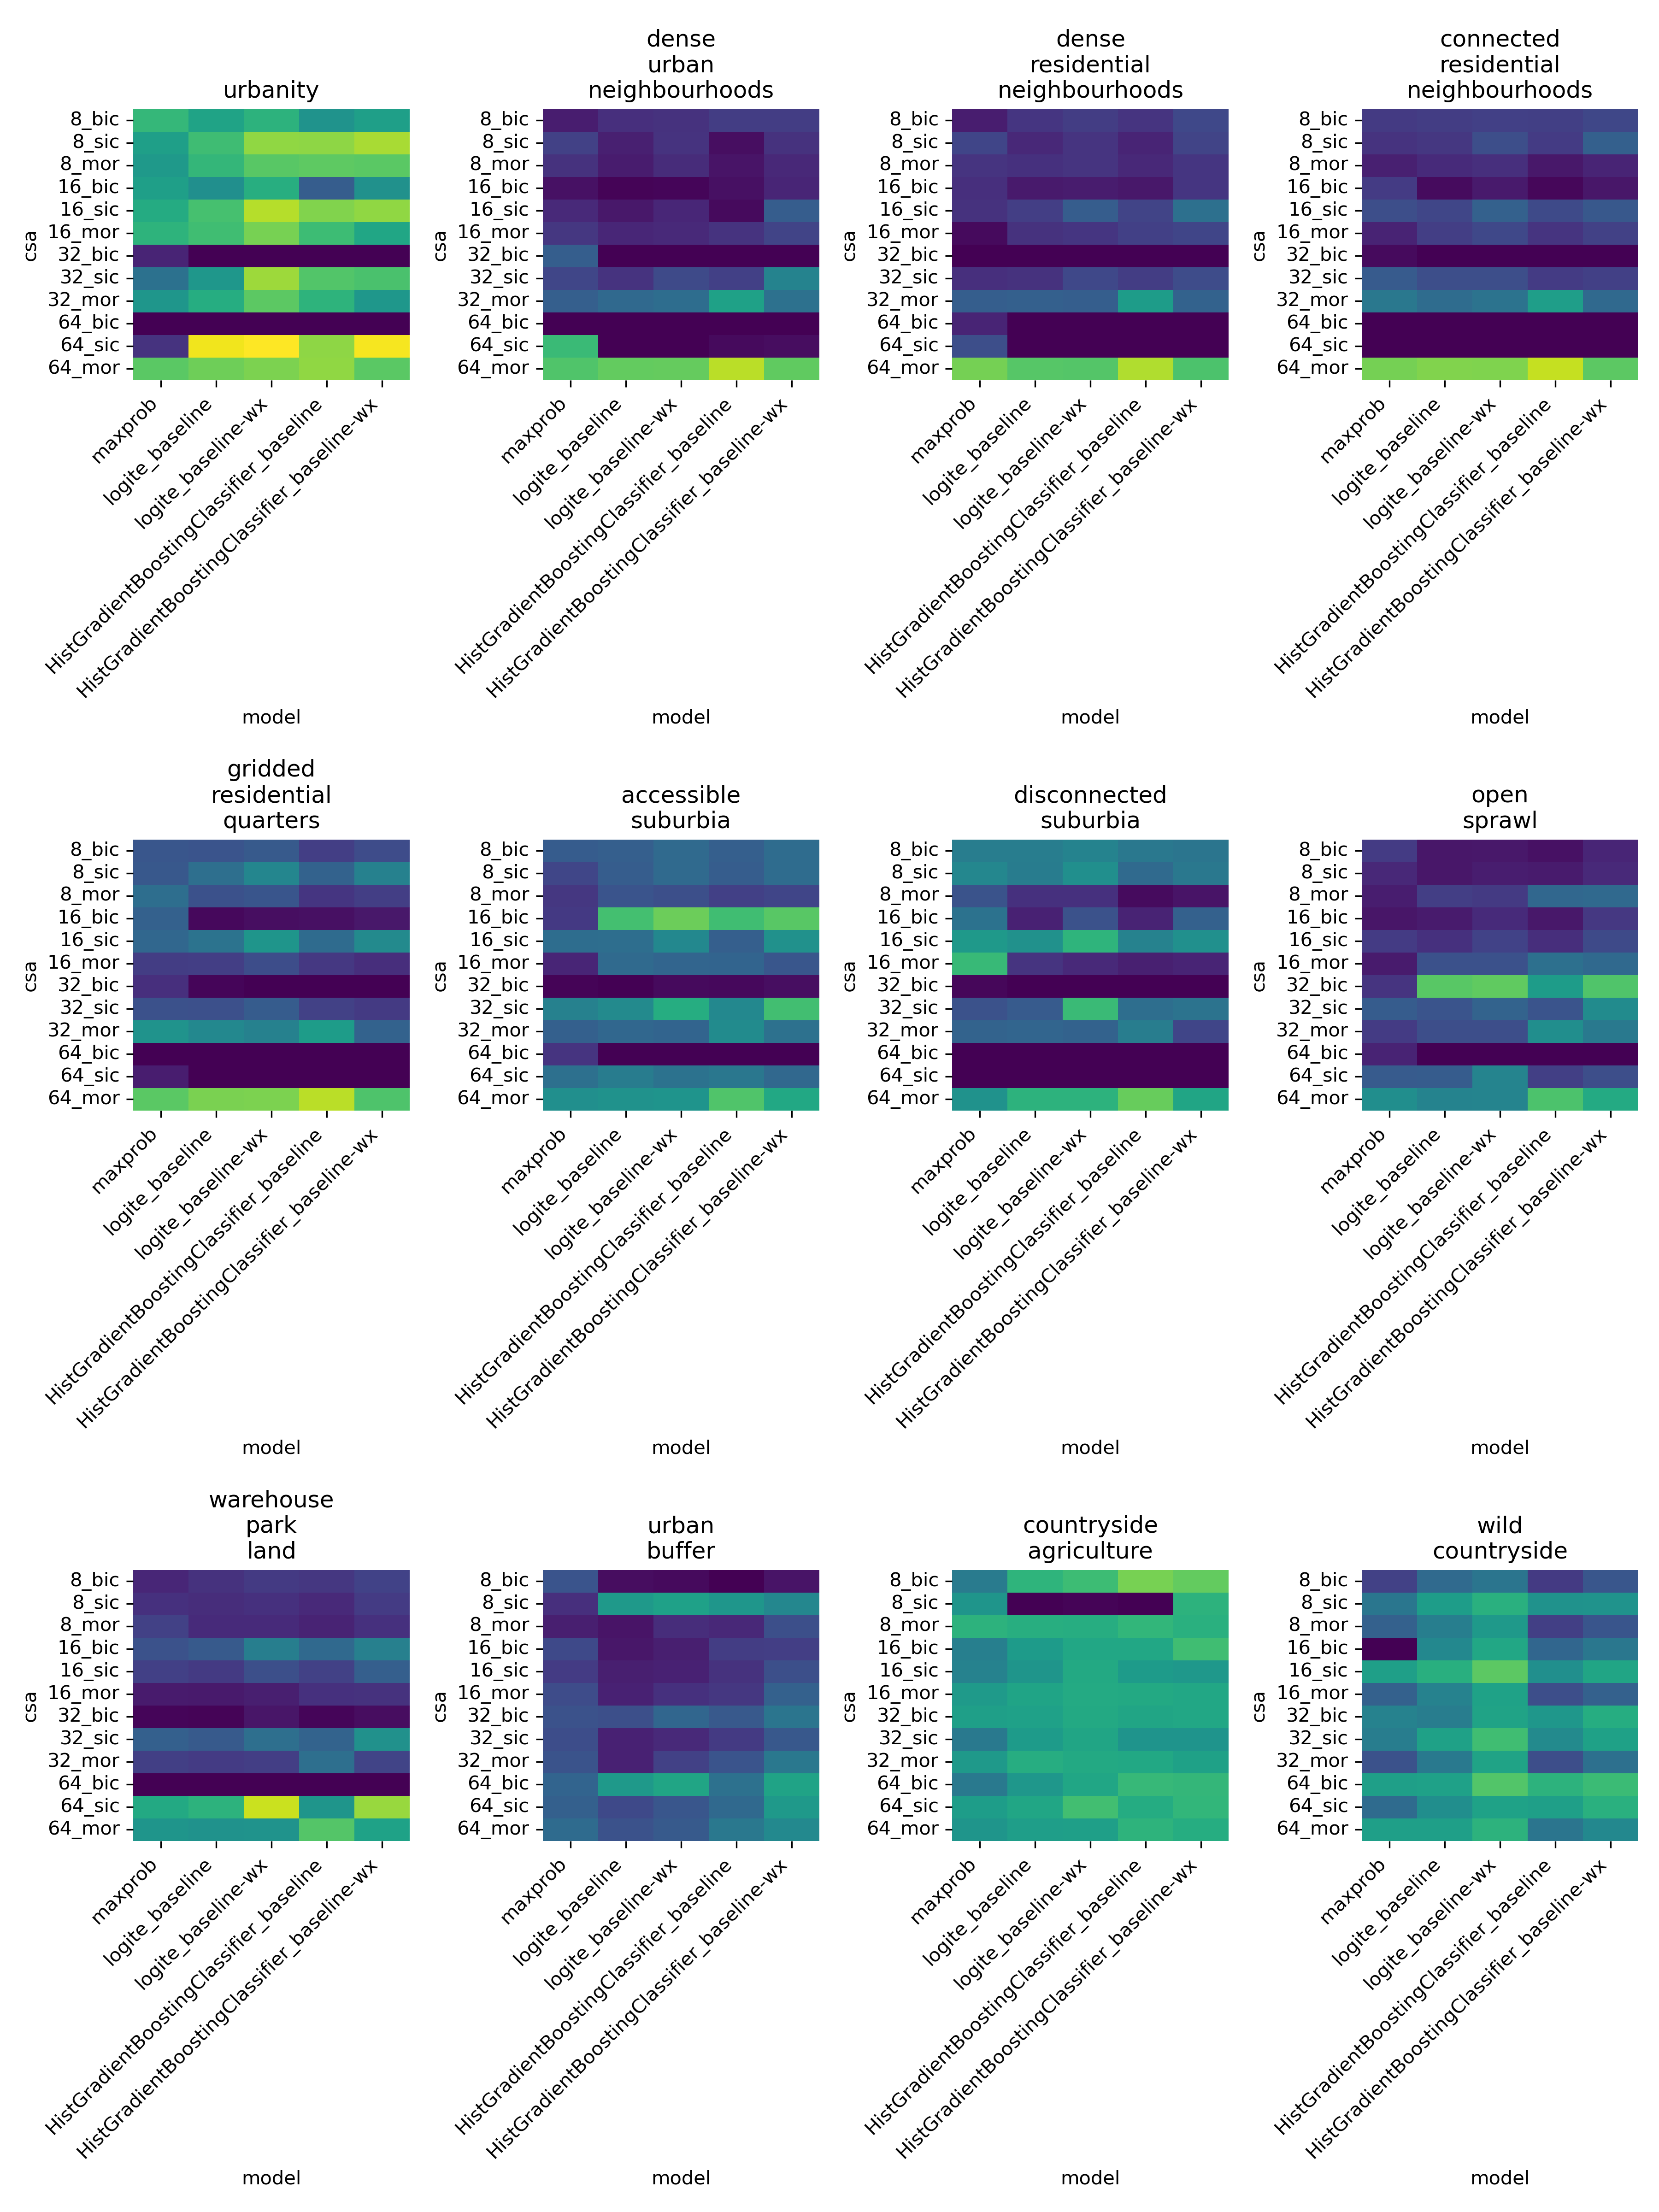
\includegraphics[width=0.8\linewidth]{wc_accuracy_x_signature.png}
    \caption{Within-class accuracy scores grouped by signature. Each panel
    represents results from one of the 12 signatures predicted. Each column in
    the heatmap
    corresponds to one of the five models compared, namely:
    histogram-based boosted classifier (\texttt{HGBC}) with features
    pertaining only to a given chip (\texttt{baseline}) or including also features
    from neighbouring ones (\texttt{baseline-wx}); Logit ensemble
    (\texttt{logite}) with the same two variations; and a simpler maximum
    probability approach (\texttt{maxprob}). Each row
    corresponds to a pair of chipsize (8, 16, 32, and 64 pixels)
    and architecture (baseline image classification, or \texttt{bic}; sliding
            image classification, or \texttt{sic}; and multi-output
    regression, or \texttt{mor}) used in the neural network stage of the
    pipeline.}
    \label{fig:wc_accuracy_x_signature}
\end{figure}

\pagebreak

\subsection{Confusion matrices}
\label{sec:appendixC}

\begin{figure}
    \centering
    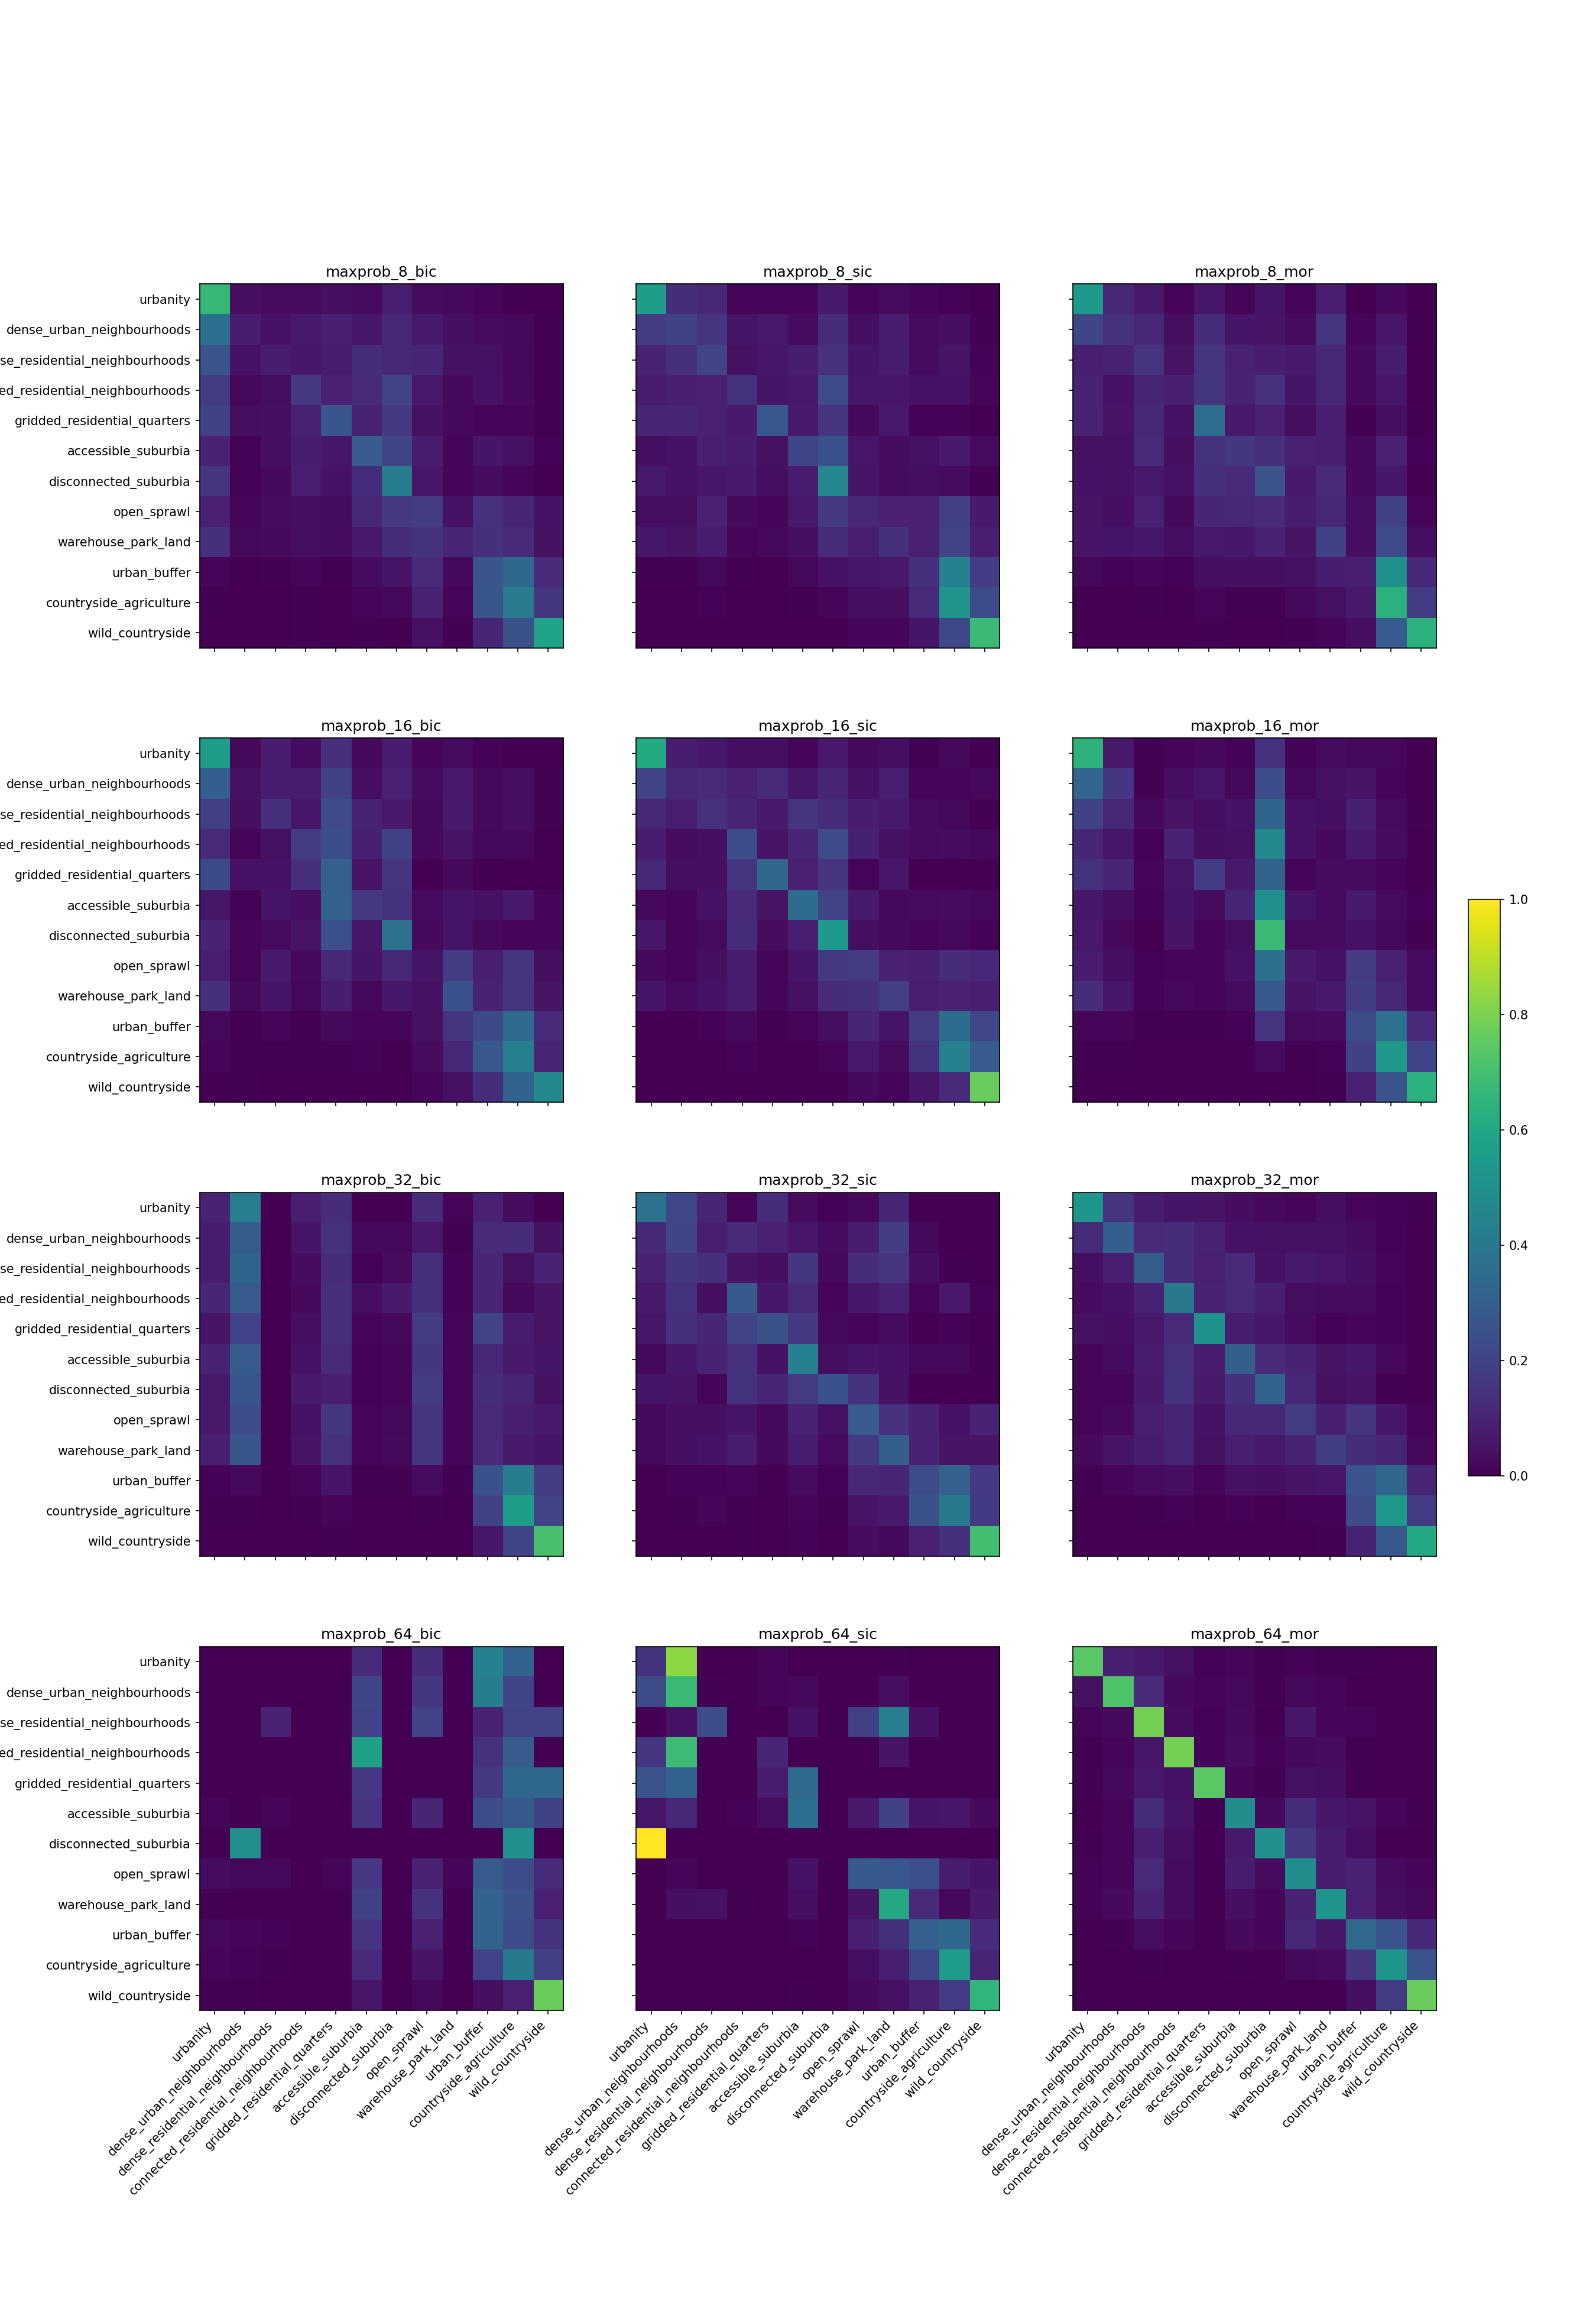
\includegraphics[width=.9\linewidth]{maxprob_cm.png}
    \caption{Confusion matrices for individual models denoting
    the ability of each model in prediction of a correct label per each class
    using the maximum probability architecture.}
    \label{fig:maxprob_cm}
\end{figure}


\begin{figure}
    \centering
    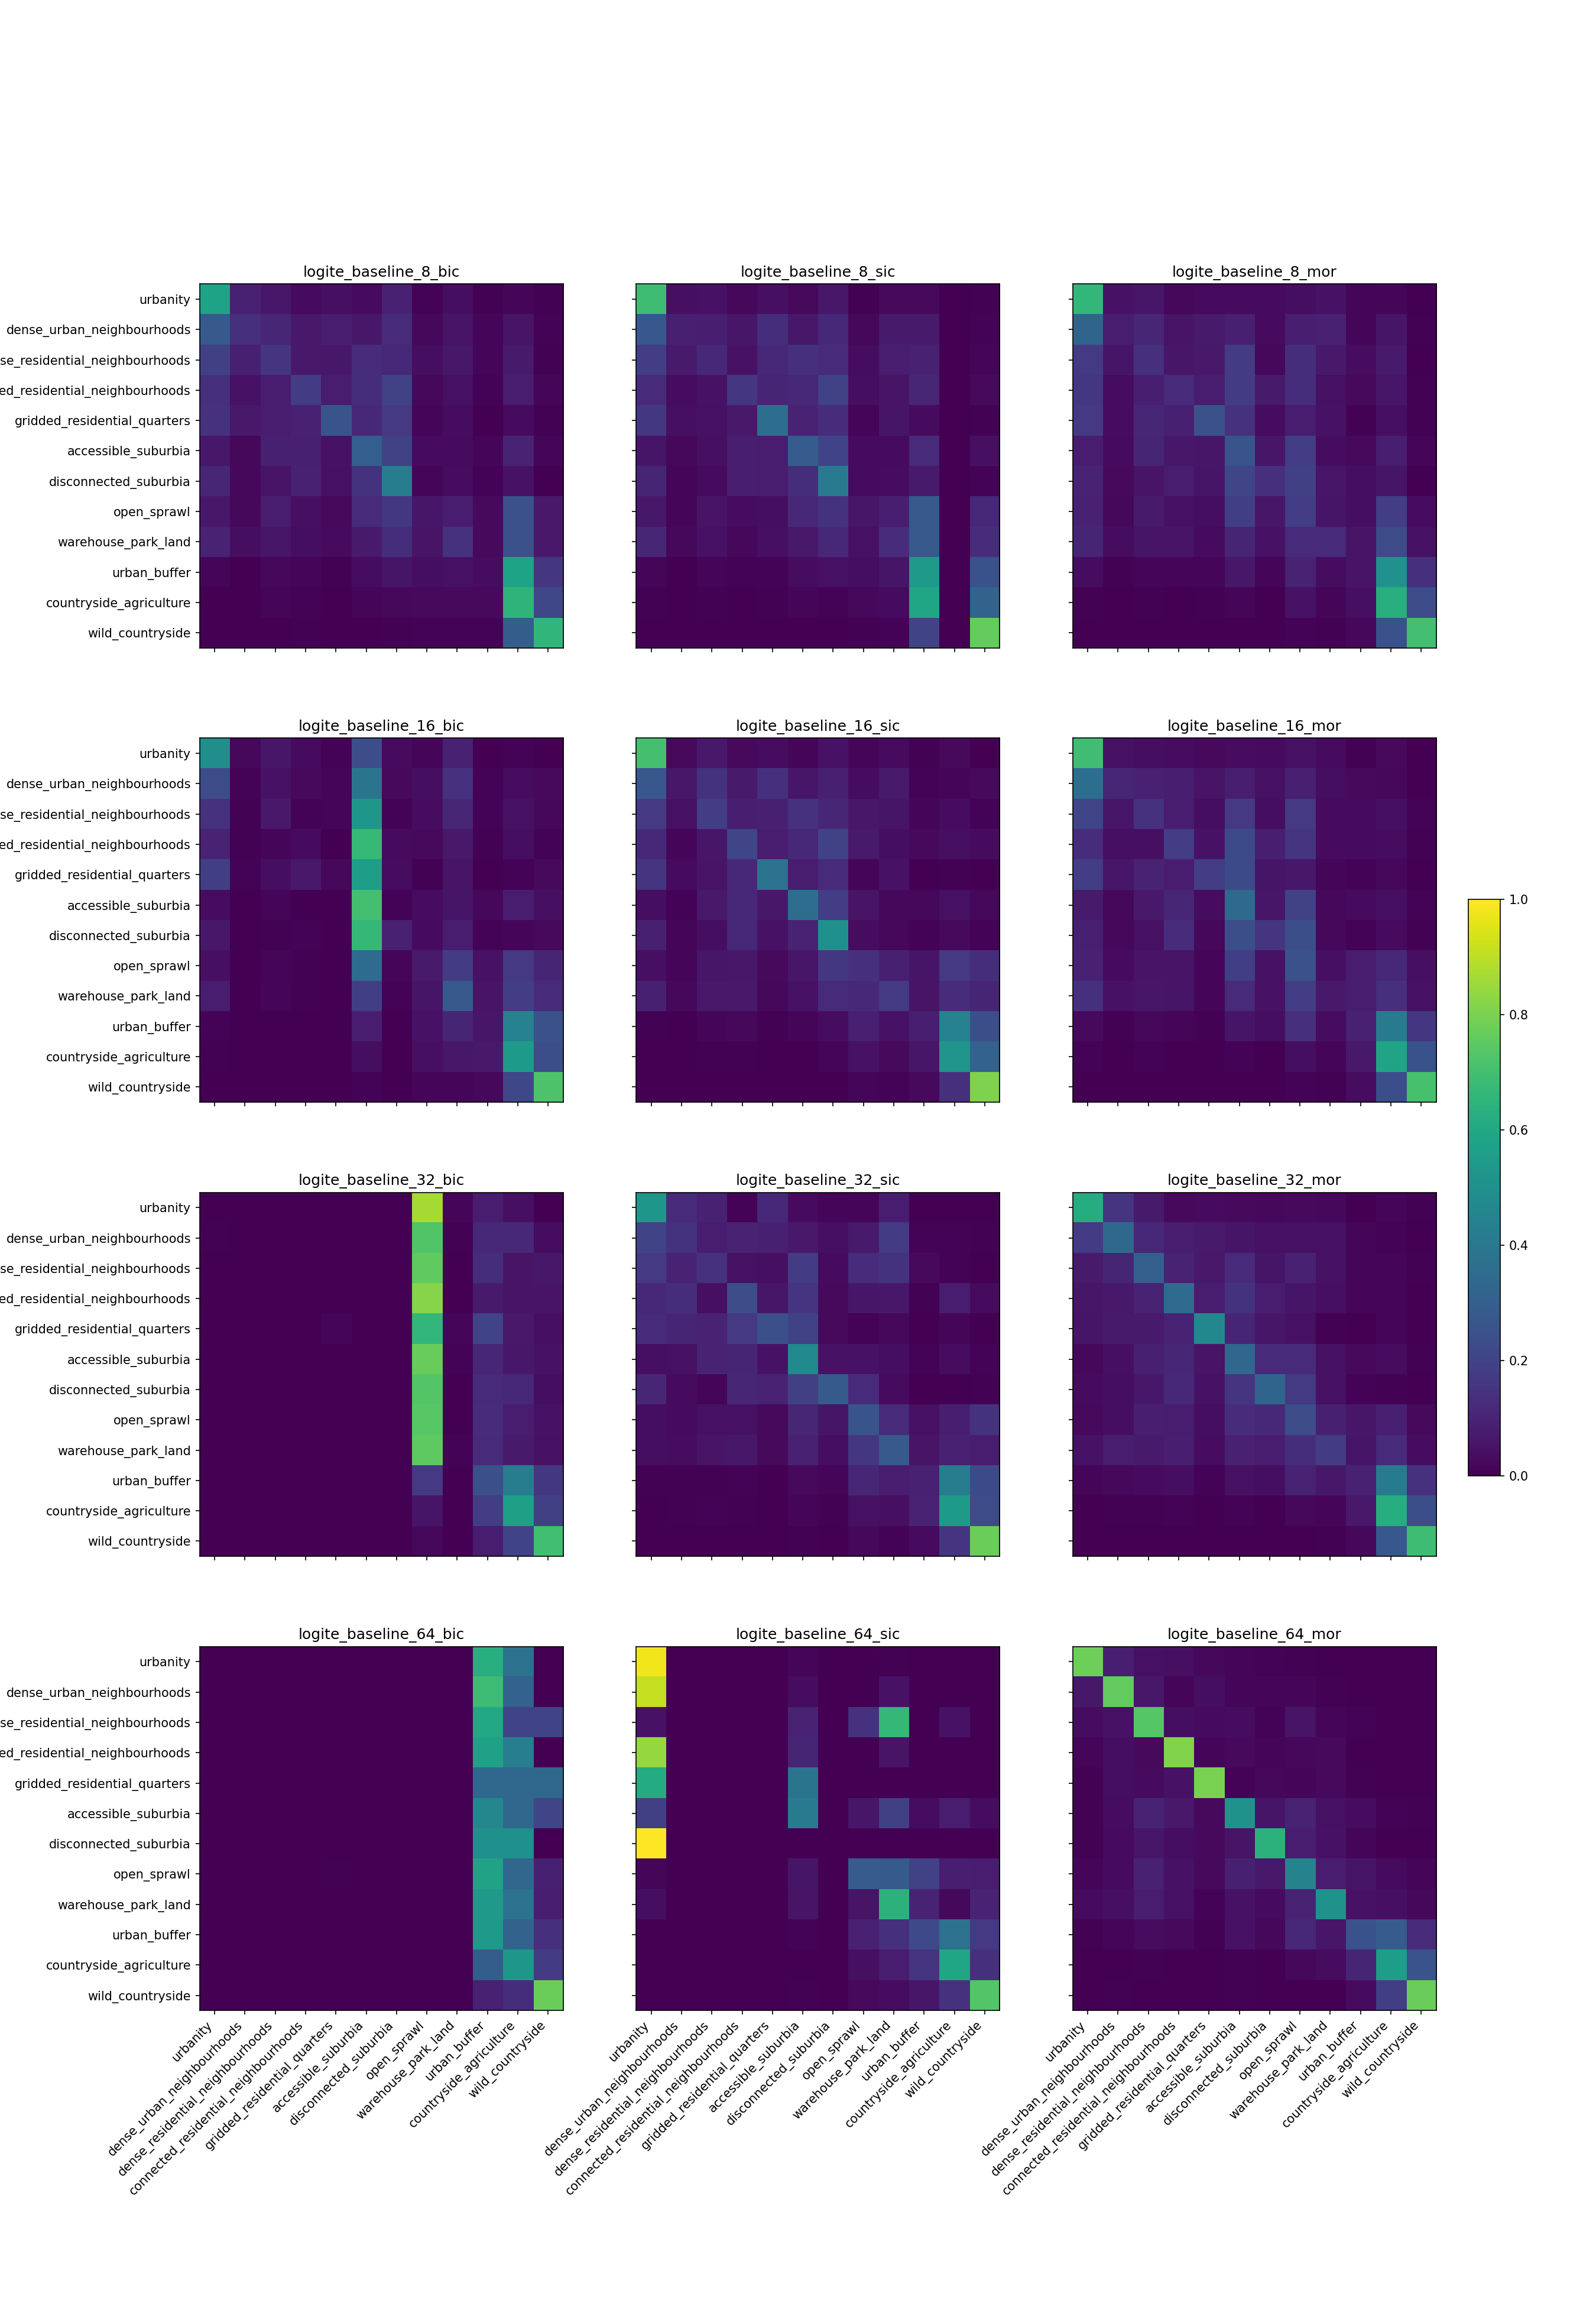
\includegraphics[width=.9\linewidth]{logite_baseline_cm.png}
    \caption{Confusion matrices for individual models denoting
    the ability of each model in prediction of a correct label per each class
    using the logit ensemble baseline architecture.}
    \label{fig:logite_baseline_cm}
\end{figure}


\begin{figure}
    \centering
    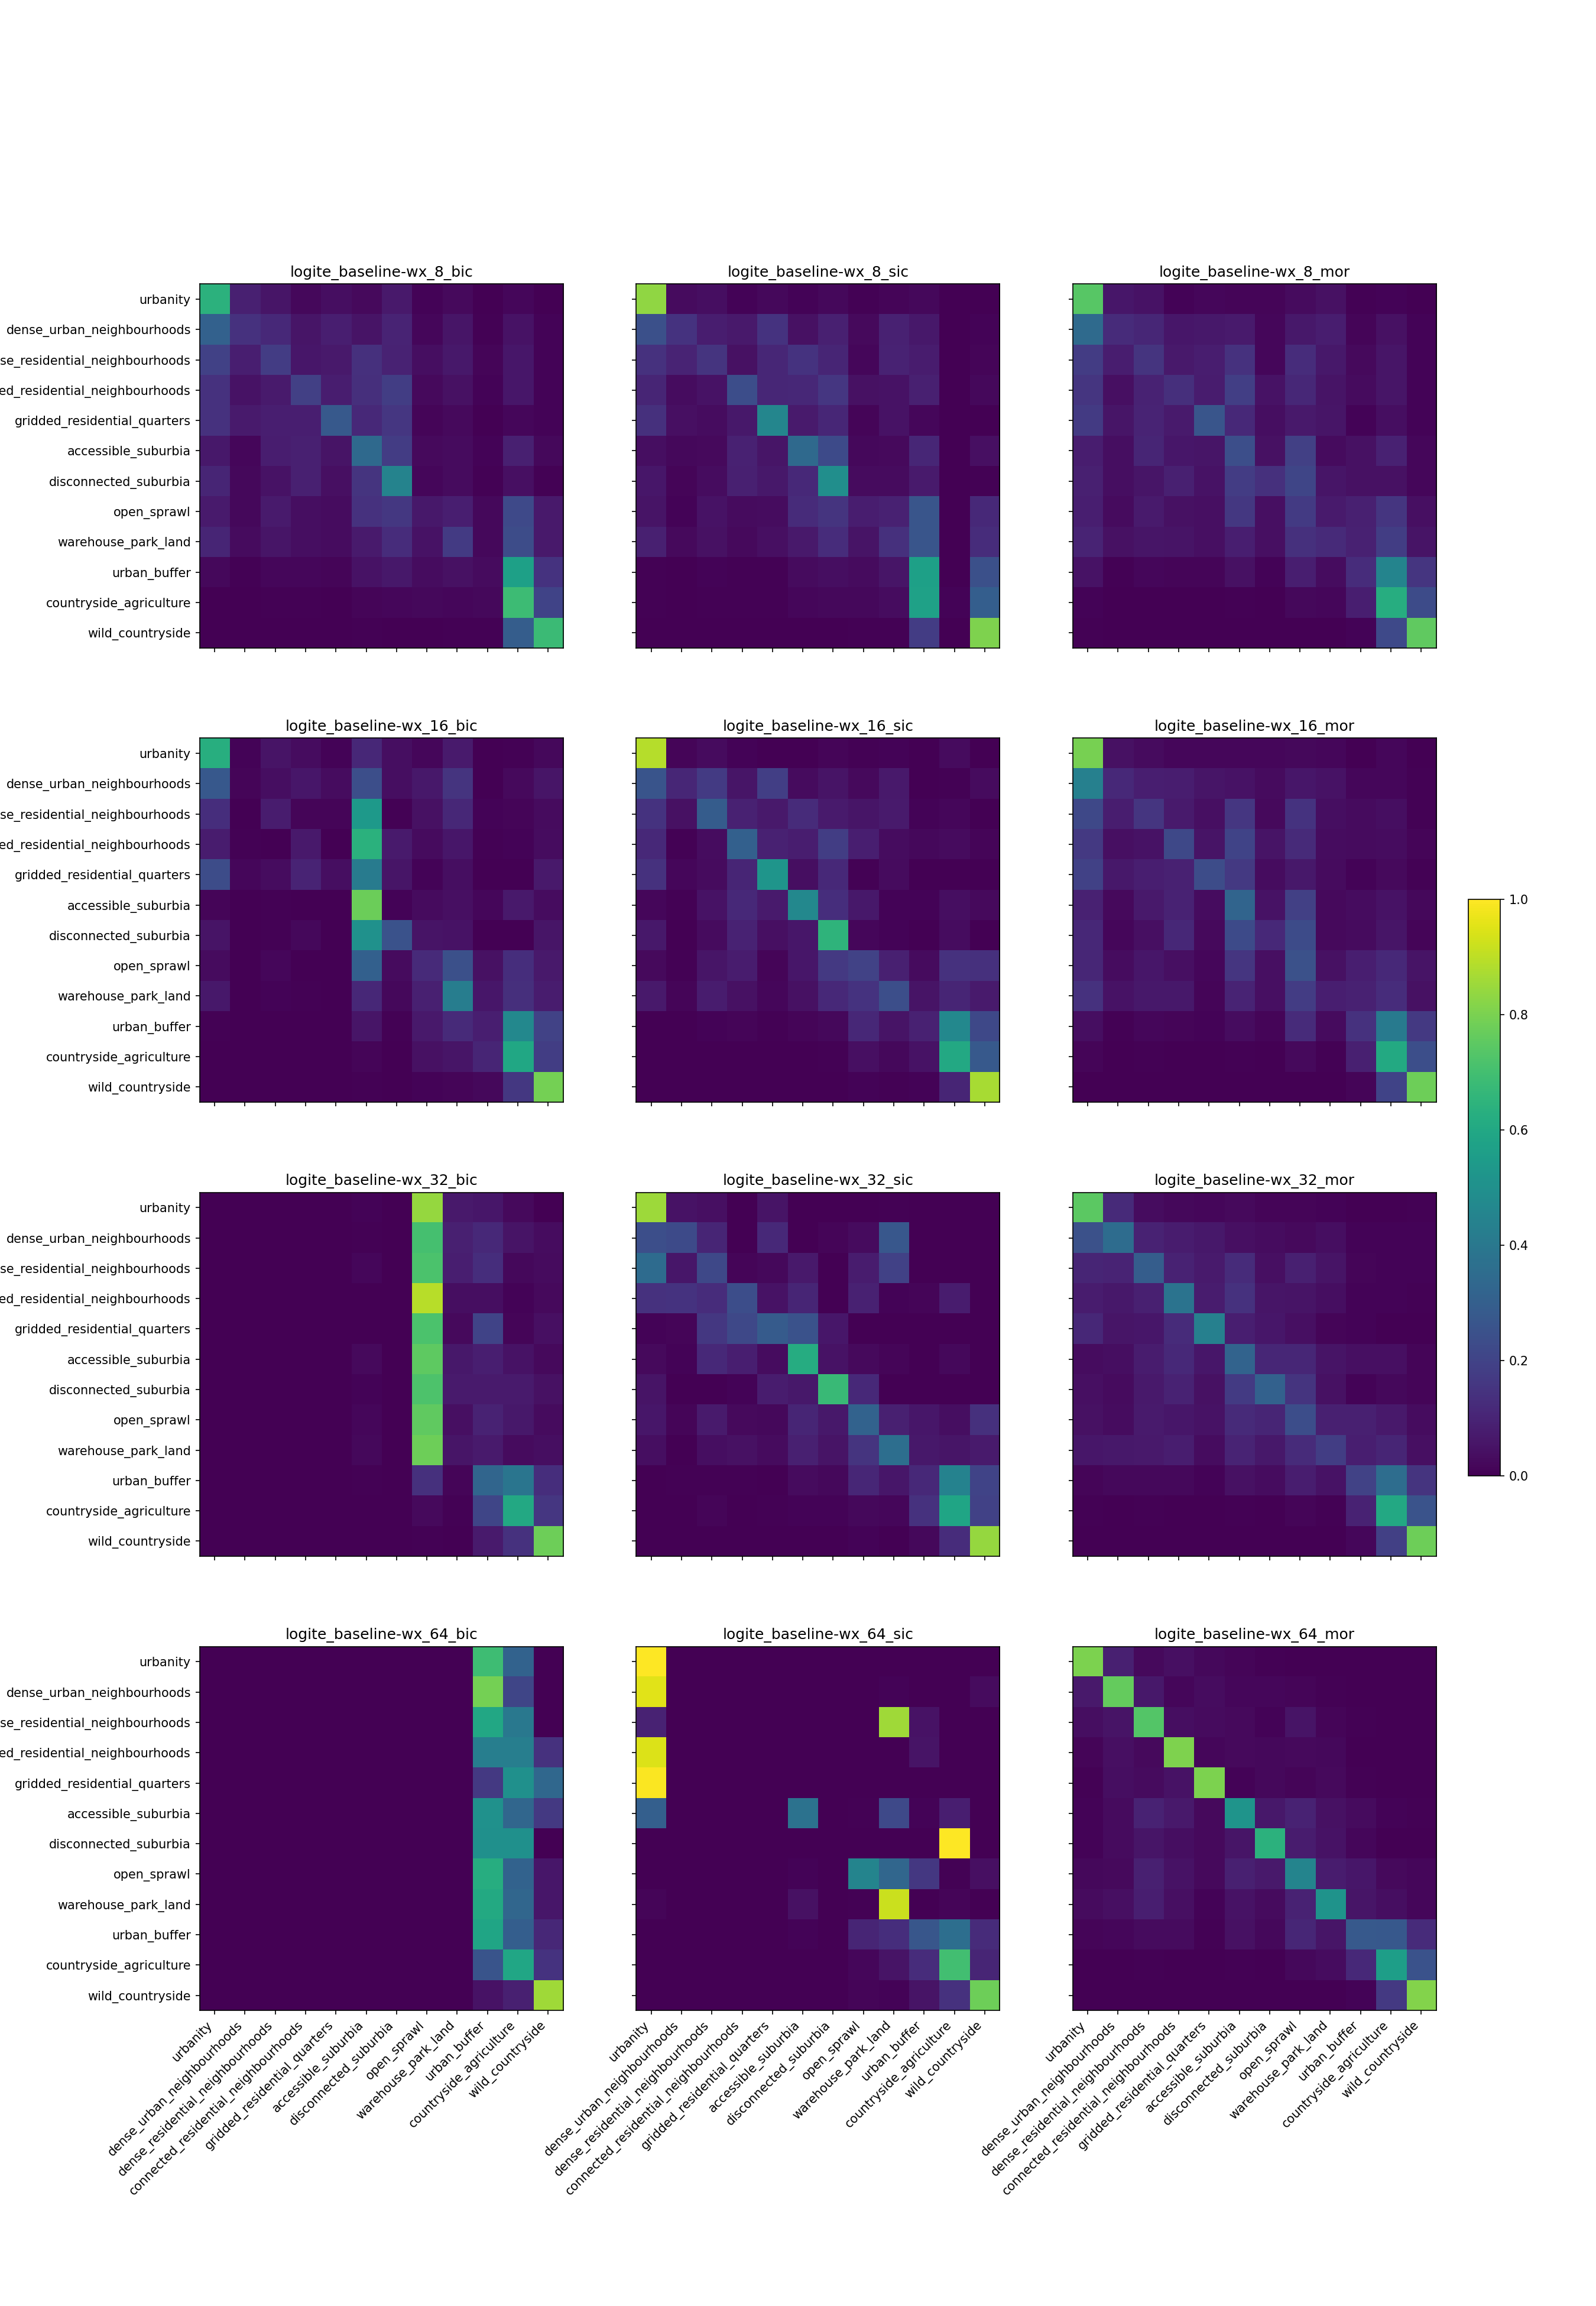
\includegraphics[width=.9\linewidth]{logite_baseline_wx_cm.png}
    \caption{Confusion matrices for individual models denoting
    the ability of each model in prediction of a correct label per each class
    using the logit ensemble baseline-wx architecture.}
    \label{fig:maxprob_cm}
\end{figure}


\begin{figure}
    \centering
    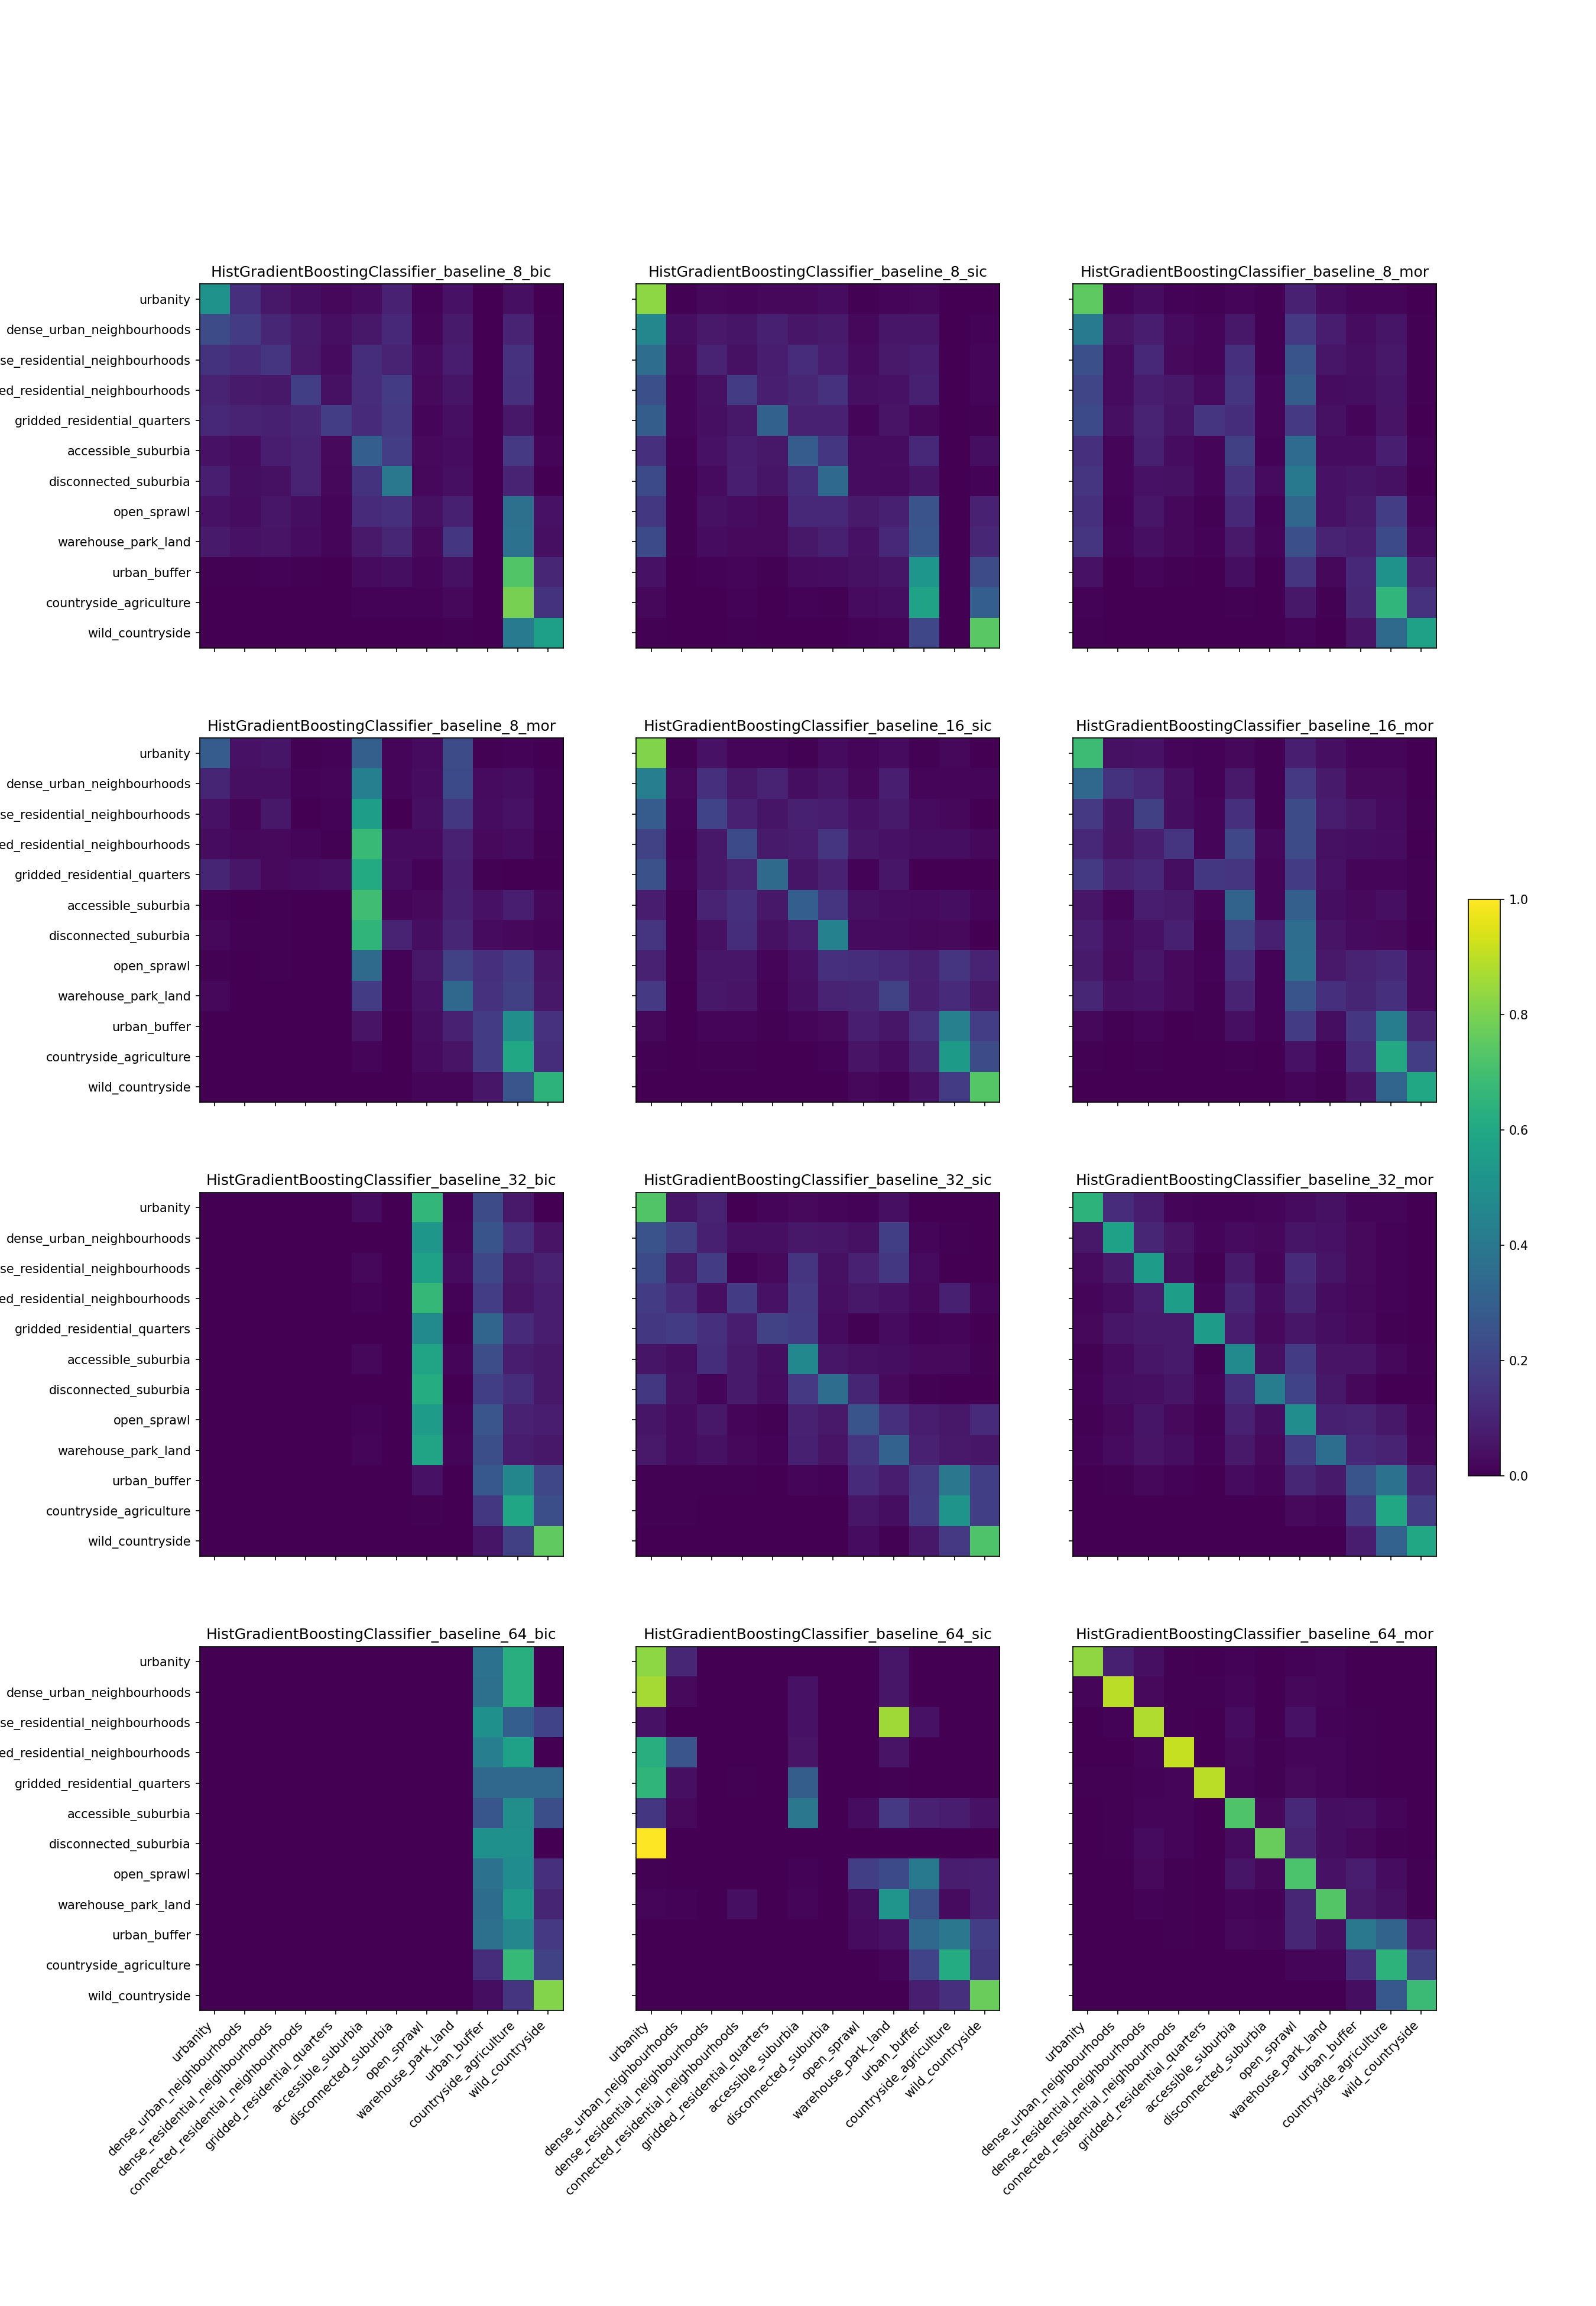
\includegraphics[width=.9\linewidth]{HistGradientBoostingClassifier_baseline_cm.png}
    \caption{Confusion matrices for individual models denoting
    the ability of each model in prediction of a correct label per each class
    using the HGBC baseline architecture.}
    \label{fig:HistGradientBoostingClassifier_baseline_cm}
\end{figure}



\begin{figure}
    \centering
    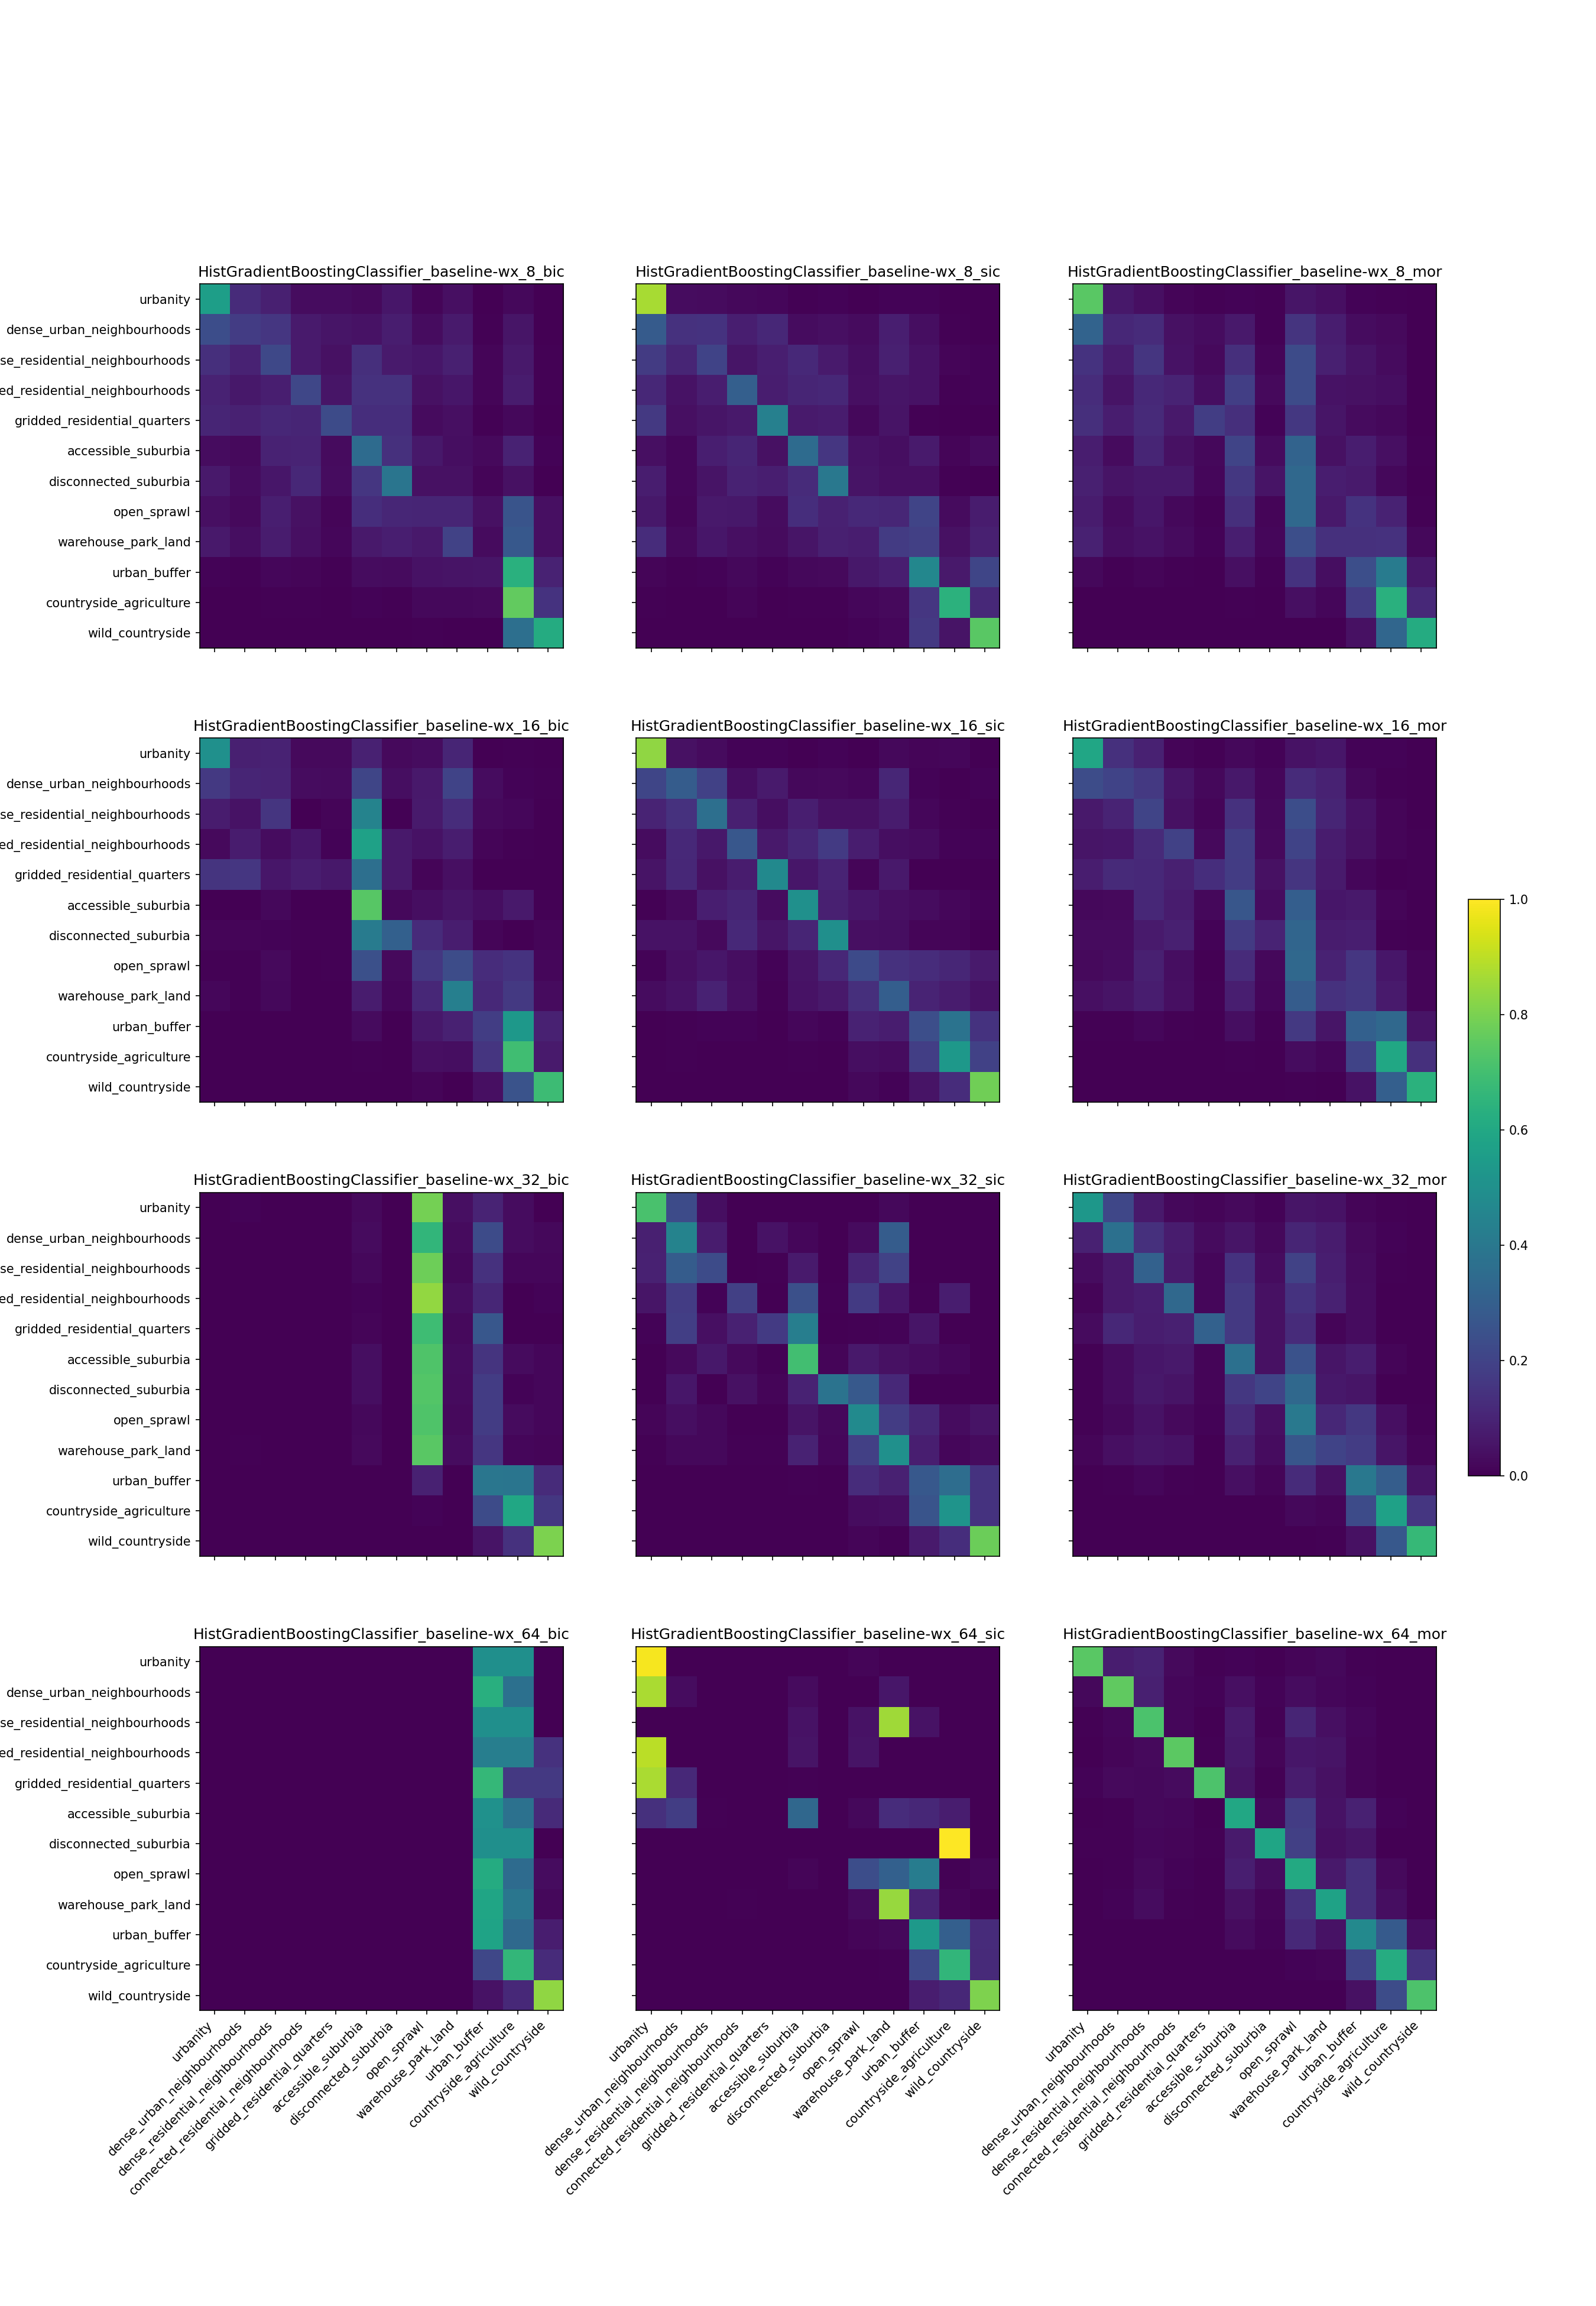
\includegraphics[width=.9\linewidth]{HistGradientBoostingClassifier_baseline_wx_cm.png}
    \caption{Confusion matrices for individual models denoting
    the ability of each model in prediction of a correct label per each class
    using the HGBC baseline-wx architecture.}
    \label{fig:HistGradientBoostingClassifier_baseline-wx}
\end{figure}



\end{document}
